\part{Part 4: Applications}

\graphicspath{ {./Pictures/} }
\chapterimage{chapter_head_2.pdf} % Chapter heading image

%++++++++++++++++++++++++++++++++++++++++++++++++++++++++++++++
\chapter{Introduction}
%++++++++++++++++++++++++++++++++++++++++++++++++++++++++++++++
\section{Gmsh}
%++++++++++++++++++++++++++++++++++++++++++++++++++++++++++++++
Gmsh is an 2D/3D finite element mesh generator included in built-in CAD engine and post-processor. Gmsh is developed in order to provide a fast, light and user-friendly meshing environment and visualization capabilities. This software is open source and the source code of Gmsh for various operating platforms (i.e. Windows, Mac and Unix) can be downloaded from http://gmsh.info. Gmsh contains four modules for geometry definition, meshing, solving and post-processing. each module has its own specifications as input and it can be controlled and manipulated interactively using the graphical user-interface (GUI), Gmsh's own scripting language (.geo file) or even using the C++, C or Python Application Programming Interface (API).
Once we execute Gmsh, the module panel appears normally in left-hand side of window, including:
\begin{itemize}
    \item \textbf{Geometry}
    \item \textbf{Mesh}
    \item \textbf{Solver}
\end{itemize}
Now, we try to explain each module separately and explain important features for each of them. The \textbf{Geometry} is a module that you can design your own geometry or import CAD design. A geometry is Gmsh is defined using its Boundary representation. It means a volume is made up of different surfaces, and each surface is made up of different curvatures or lines. Then, each curvature or line is bounded by two end points. Therefore, this representation shows the way we should take to design a 2D/3D geometry.
Therefore, to define a shape in space, set of points are specified and the connections between these pints are built by straight lines or curvatures. Now, Gmsh can figure out surfaces based on the boundaries defined (line/curvature/end point). Later, based on the surfaces defined, Gmsh ca generates volume of geometry in space.

This module has some sections that help you to define geometric parameters and shape of your design. Some of important sections of this module is enlisted and described as follows:
\begin{itemize}
    \item \textbf{Elementary entities}: helps to add, merge, split or delete points, lines, curves, faces or volumes we defined.
    \item \textbf{Physical groups}: manages boundary conditions and physical properties (i.e. fluid or solid) of predefined geometry.
    \item \textbf{Reload script}: reads and load the data defined predefined geometry from Gmsh's own language script saved in .geo file.
    \item \textbf{Edit script}: allows you to edit the .geo file manually to change any specifications.
\end{itemize}
It is worth pointing out that all specifications of geometry are saved in .geo file, this helps operator to manually manipulate geometry or any other specifications. 
After building geometry and defining boundary conditions via \textbf{Geometry} module, the next step is to make finite element mesh of the geometry model using \textbf{Mesh} module. This module helps to define our geometry model by simple geometrical elements, such as: lines, triangles, tetrahedra, hexahedra and pyramids. Gmsh uses different algorithms for generating mesh automatically and the type of mesh in Gmsh is unstructured by default, otherwise we specify to generate structured one. \textbf{Mesh} module has also some sections that help to specify the type, number and density of mesh in domain. Here, some of important sections are provided as follows:
\begin{itemize}
    \item \textbf{Define}: sets number of grids as well as growth ratio on the boundaries. Additionally, it specifies the mesh type (whether Structured or Unstructured).
    \item \textbf{2D/3D}: makes mesh for surfaces/volumes existed in domain. It automatically generate mesh based on the specifications provided in \textbf{Define} section.
    \item \textbf{Set order 1, 2, or 3}: Since the grid points in the mesh are connected to each other by straight lines (\textbf{Set order 1}), sometimes it is inefficient to define a geometry's curvatures using these straight lines. However, to overcome this problem, the mesh lines that define these curvatures can be more flexible and defined as polynomial (\textbf{Set order 2 or 3}). This feature helps to have more smooth mesh just beside curvatures to increase mesh quality in these regions.
    \item 
\end{itemize}
Additionally, there is another module named \textbf{Solver}, which embed Gmsh directly to another solver.
In this section, we are trying to explain how to use Gmesh in order to design and build a mesh-file for CFD application. This module makes an interface to share parameters and modeling information with different solvers. ONLAB (http://onelab.info) is one of examples that is used for this purpose. Explaining more details about this module is beyond the scope of this book.
%++++++++++++++++++++++++++++++++++++++++++++++++++++++++++++++
\section{SU2}
%++++++++++++++++++++++++++++++++++++++++++++++++++++++++++++++
\section{Paraview}
%++++++++++++++++++++++++++++++++++++++++++++++++++++++++++++++
\chapter{Inviscid NACA 0012}
%++++++++++++++++++++++++++++++++++++++++++++++++++++++++++++++
\section{Problem Description}
In this tutorial, we are going to explain how to simulate inviscid flow around an NACA0012 airfoil. Since the flow is assumed to be inviscid, we apply Euler equation for flow modeling. Please note that at high Reynolds numbers, the flow could be assumed to be inviscid, since viscosity term in Navier-Stokes equations becomes negligible. For this example, the flow specifications are provided as follows:
\begin{itemize}
    \item Pressure = 101,325 Pa
    \item Temperature = 273 K
    \item Mach number = 0.8
    \item Angle of attack = 1.25 degree
\end{itemize}
The tutorial has two parts: Flow Solution and Post-Processing. In the first part, we explain how to manage prerequisite files and settings, and how to run the CFD simulation using SU2. In the second part, we explain how to use Paraview software to visualize data obtained form SU2.
%++++++++++++++++++++++++++++++++++++++++++++++++++++++++++++++
\section{Flow solution}
To run the simulation, the SU2 needs two essential files: configuration file (.cfg) and mesh file (.su2). In this example, the following files are located in \textit{01Quickstart} folder:
\begin{enumerate}
\item \textit{inv\_NACA0012}.cfg as a configuration file.
\item \textit{mesh\_NACA0012\_inv}.su2 as a mesh file.
\end{enumerate}
The next step is to copy these two files in directory of SU2, where the execution and script files are located there. To run this simulation, open the command line terminal and enter the following commands:
\begin{table}[htbp]
    \centering
    \begin{tabular}{|l|l|}
    \hline
    Windows     & \begin{tabular}{c} \$ cd "where you saved the package" \\ \$ SU2\_CFD.exe inv\_NACA0012.cfg \end{tabular}
    \\
    \hline
    OSX     & \begin{tabular}{c} \$ cd "where you saved the package" \\ \$ SU2\_CFD.exe inv\_NACA0012.cfg \end{tabular}
    \\
    \hline
    \end{tabular}
\end{table}

The SU2 solver will commence calculation and print out the residuals at every iteration until the specified convergence criteria is achieved. After calculations are done, the following output files should be generated and saved in the SU2 folder:
\begin{itemize}
    \item \textit{flow}.vtk: contains the full volume flow solution.
    \item \textit{force\_breakdown}.dat: contains forces and moment on the airfoil.
    \item \textit{history}.vtk: contains convergence history of calculations.
    \item \textit{restart\_flow}.dat: for restarting simulation.
    \item \textit{surface\_flow}.vtk: flow solution on the surface of the airfoil.
    \item \textit{surface\_flow}.csv: comma separated values of flow solution on the airfoil (If you want to plot data in another software, like Microsoft Excel, you can use this file).
\end{itemize}
Please keep in mind that every time you run SU2, the output data will be overwritten. Hence, before launching new simulation, you could make a new folder and transfer your data from previous simulation to this folder.
%++++++++++++++++++++++++++++++++++++++++++++++++++++++++++++++
\section{Post-processing}
In this section, we explain how to use Paraview to visualize CFD data for this example. First of all, install Paraview (this tutorial uses Paraview 3.12.0) if you do not have it on your computer. Otherwise, take following steps for visualization:
%--------------------------------------------------------------
\subsection{Load Solution File:}
Launch Paraview. Go to \textbf{File} $\rightarrow$ \textbf{Open}, and then select \textit{flow}.vtk file. On the left-hand side of Paraview window you will see the file appears under \textbf{builtin} in \textbf{Pipeline Browser}. Now press \textbf{Apply} button in \textbf{Properties} tab, just right under the  \textbf{Pipeline Browser}. After taking these steps, your file is loaded by software and is ready to visualize (Fig.\ref{fig:load}).
\begin{figure}[htbp]
    \centering
    \includegraphics[width=0.4\textwidth]{tut01/loadvtkfile.pdf}
    \caption{Loading .vtk file in the \textbf{Pipeline Browser}.}
    \label{fig:load}
\end{figure}
%--------------------------------------------------------------
\subsection{Visualize Mesh Domain}
In order to view mesh, according to Fig.\ref{fig:wireframe}, select \textit{Solid Color} with \textit{Wireframe} in the toolbar. Then, you can zoom in to see mesh around the airfoil like Fig.\ref{fig:mesh}. As you can see, the mesh around the NACA0012 is unstructured, and the grids are clustered around the leading and trailing edges of the airfoil.
\begin{figure}[htbp]
    \centering
    \includegraphics[width=0.6\textwidth]{tut01/wireframe.pdf}
    \caption{How to display mesh in computational domain.}
    \label{fig:wireframe}
\end{figure}
\begin{figure}[htbp]
    \centering
    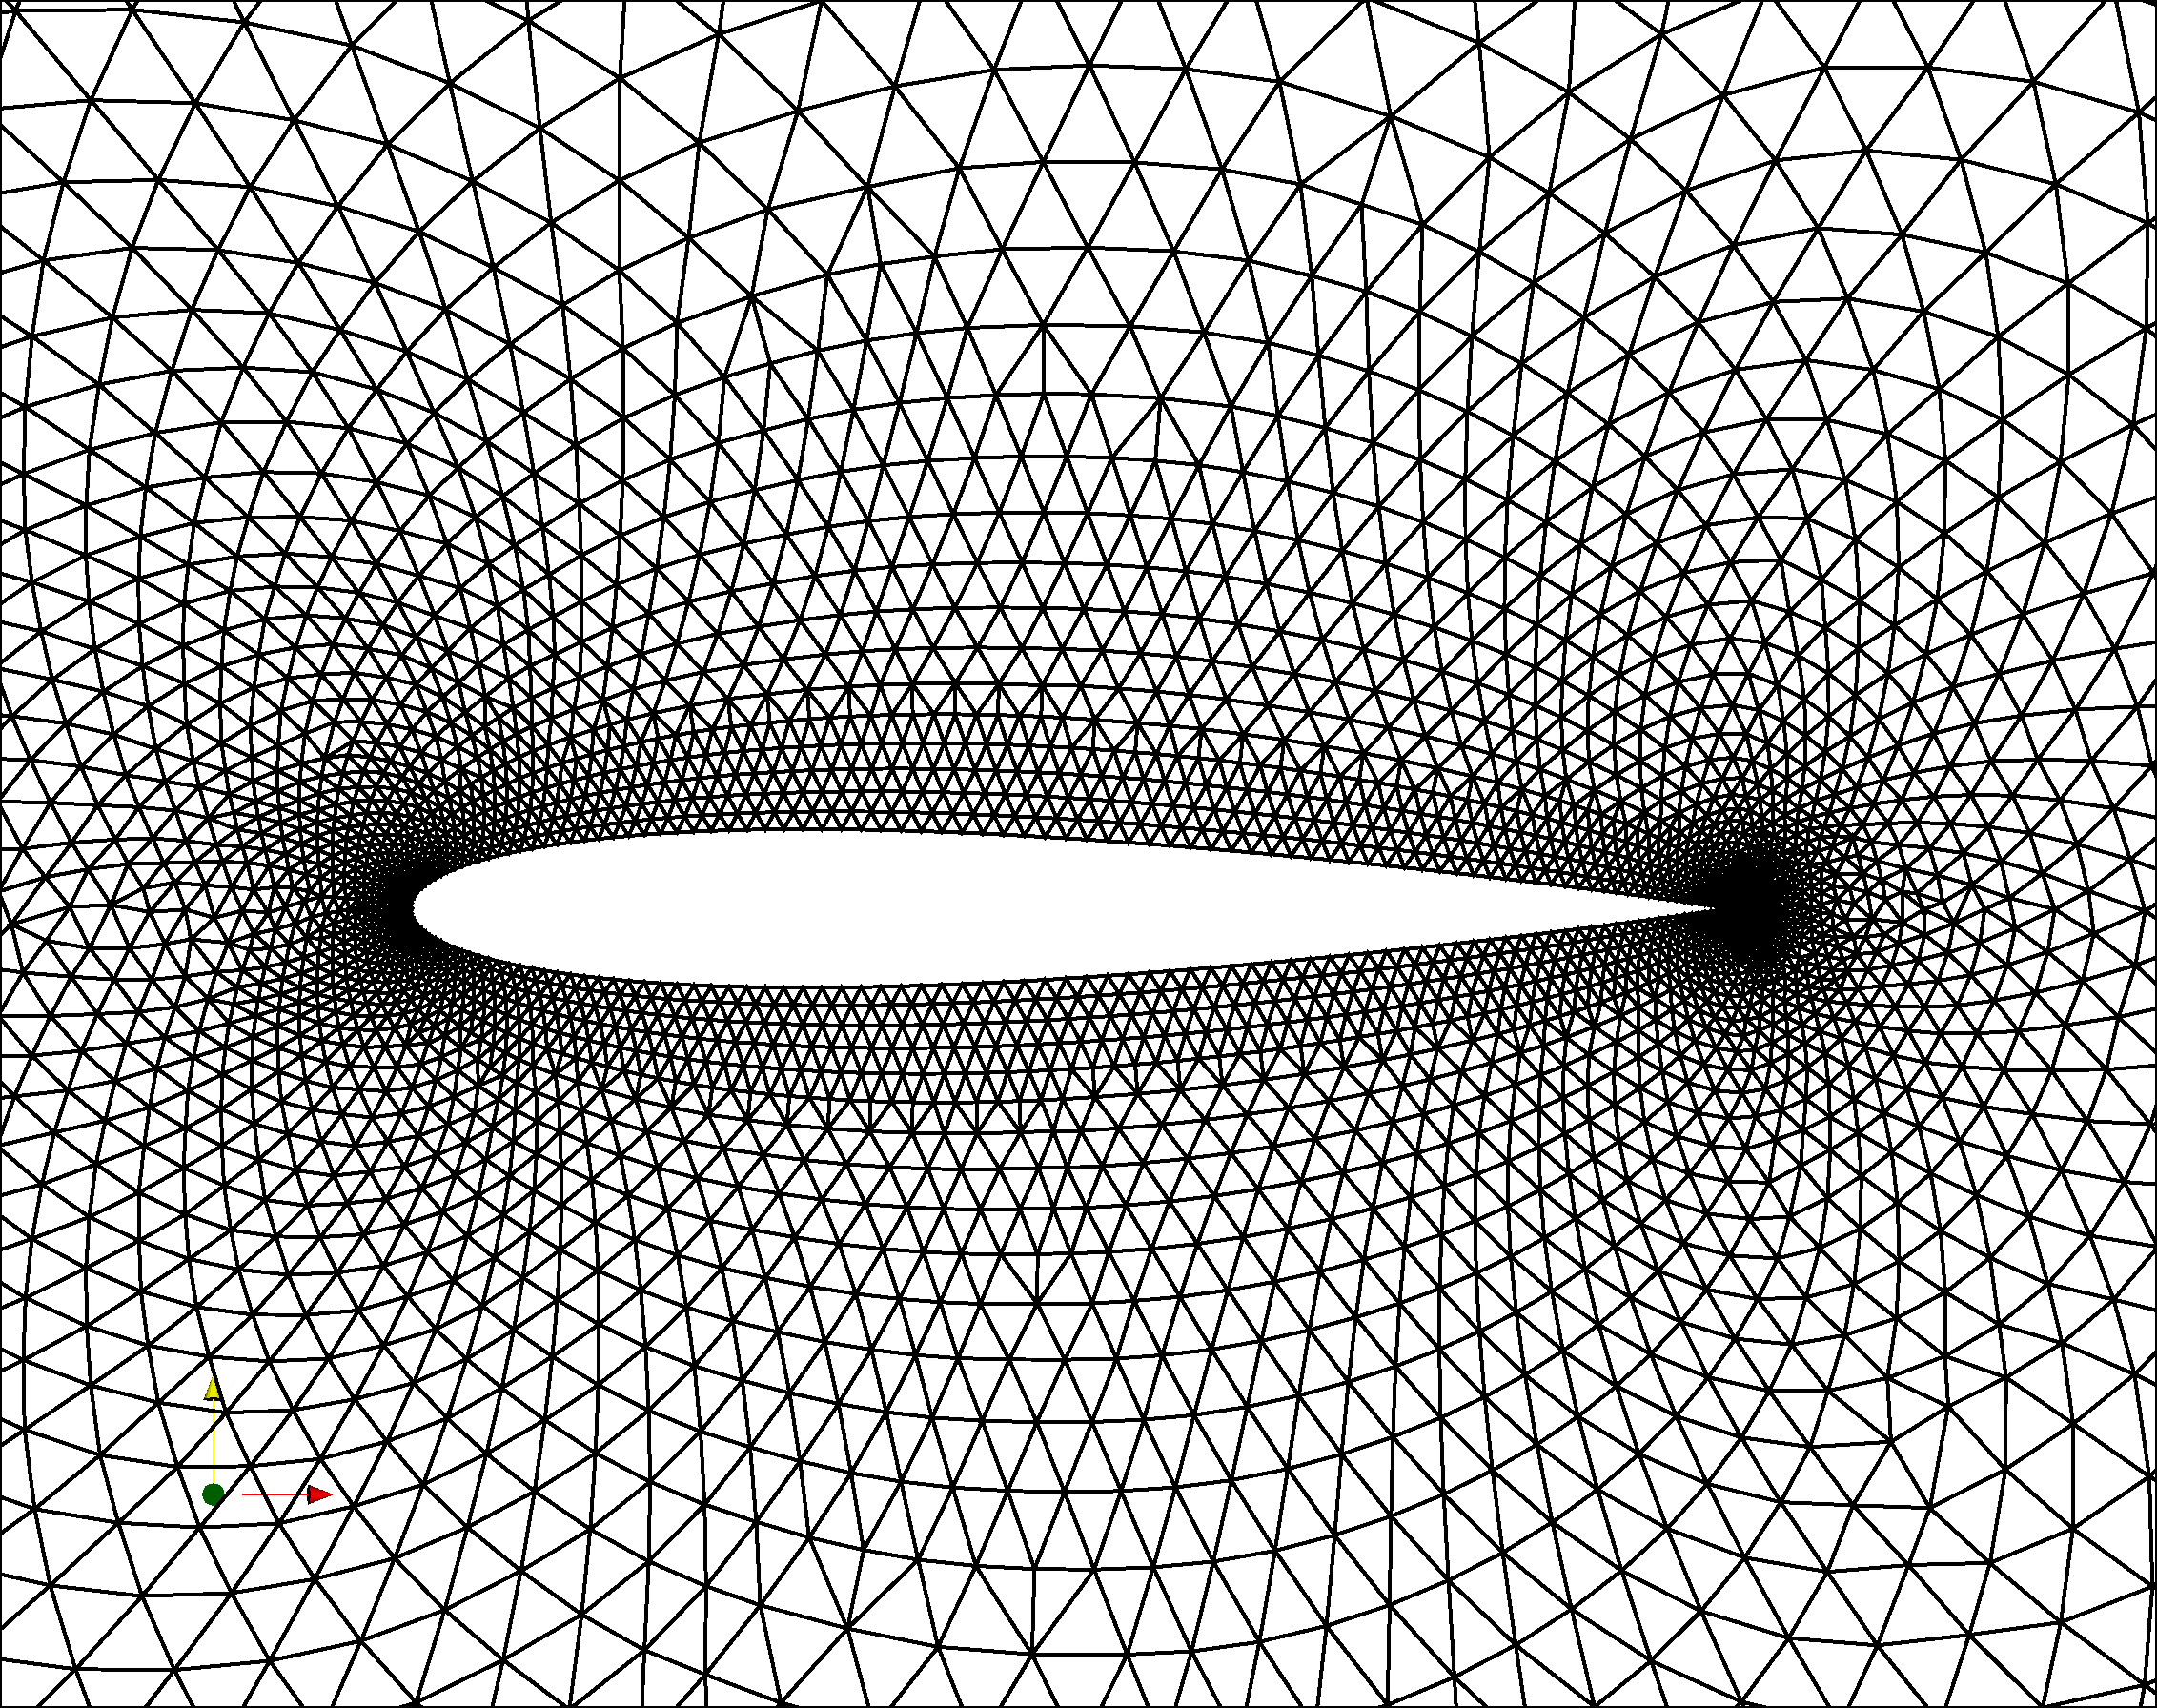
\includegraphics[width=.75\textwidth]{tut01/mesh.pdf}
    \caption{Unstructured mesh around NACA0012.}
    \label{fig:mesh}
\end{figure}
%--------------------------------------------------------------
\subsection{Visualize Pressure Contour}
In order to visualize pressure contour, click on the \textit{flow}.vtk from \textbf{Pipeline Browser} to activate the file, and then click on the \textbf{Properties} tab. According to Fig.\ref{fig:colorby}, in \textbf{Coloring} section, select \textit{Pressure} from drop-down menu. To change color settings for the pressure, you can also click on the \textbf{Edit} under the \textbf{Coloring}. Normally another display window appears on the right-hand side of the monitor, similar to Fig.\ref{fig:change_color_range}. Now you can change the maximum/minimum range of pressure to your desirable values by \textbf{Set Range}, or change contour colors by \textbf{Choose Preset} (Fig.\ref{fig:change_color_range}).
\begin{figure}[htbp]
    \centering
    \includegraphics[width=0.4\textwidth]{tut01/contourdisplay.pdf}
    \caption{Contour settings in \textbf{Display} tab.}
    \label{fig:colorby}
\end{figure}
\begin{figure}[htbp]
    \centering
    \includegraphics[width=0.5\textwidth]{tut01/colormap.pdf}
    \caption{How to change color and max/min values for contour.}
    \label{fig:change_color_range}
\end{figure}
After taking these steps, the pressure contour in the display window should be similar to Fig.\ref{fig:pressure_contour}.
\begin{figure}[htbp]
    \centering
    \includegraphics[width=.75\textwidth]{tut01/pressurecontour1.pdf}
    \caption{Pressure contour for NACA0012 airfoil.}
    \label{fig:pressure_contour}
\end{figure}

To add contour lines, click again on the \textit{flow}.vtk file in the \textbf{Pipeline Browser}, and then click on the \textbf{Contour} icon (Fig.\ref{fig:contour_icon}) in toolbar.
\begin{figure}[htbp]
    \centering
    \includegraphics[width=0.6\textwidth]{tut01/contourlineicon.pdf}
    \caption{Contour icon in toolbar.}
    \label{fig:contour_icon}
\end{figure}
Now you should see \textit{Contour1} appears under \textit{flow}.vtk file in the \textbf{Pipeline Browser} (Fig.\ref{fig:contour1}).
\begin{figure}[htbp]
    \centering
    \includegraphics[width=0.5\textwidth]{tut01/contour1.pdf}
    \caption{Adding \textit{Contour1} in \textbf{Pipeline Browser}.}
    \label{fig:contour1}
\end{figure}
According to Fig.\ref{fig:contourby a}, go to the \textbf{Properties} tab, and select \textit{Pressure} from \textbf{Contour By} drop-down menu. Next, click on the \textbf{New Range} icon to customize the range of pressure contour. For now, set the number of step to 20, similar to Fig.\ref{fig:contourby b}. It means the pressure contour range is equally divided by 20 portions, and the pressure values in each portion are limited by two lines in the display window. At the end, click on \textbf{Apply} to see contour lines in display window.
\begin{figure}[htbp]
    \centering
     \begin{subfigure}[b]{.4\textwidth}
         \centering
         \includegraphics[width=1.0\textwidth]{tut01/contourlinenewrange.pdf}
         \caption{Define new range}
         \label{fig:contourby a}
     \end{subfigure}
     \hfill
     \begin{subfigure}[b]{.4\textwidth}
         \centering
         \includegraphics[width=1.0\textwidth]{tut01/addrangepdf.pdf}
         \caption{Add range}
         \label{fig:contourby b}
     \end{subfigure}     
    \caption{How to define a new range for the contour lines.}
    \label{fig:contourby}
\end{figure}
Next, as it is shown in Fig.\ref{fig:colorby2}, click on the \textbf{Display} under \textbf{Properties} tab. In \textbf{Coloring} section, select \textbf{Solid Color} form drop-down menu, and choose white color form \textbf{Edit}.
\begin{figure}[htbp]
    \centering
    \includegraphics[width=0.6\textwidth]{tut01/coloring.pdf}
    \caption{Changing contour lines color in \textbf{Coloring} section.}
    \label{fig:colorby2}
\end{figure}
Eventually, the pressure contour with contour lines should be similar to Fig.\ref{fig:pressure_contour_lines}.
\begin{figure}[htbp]
    \centering
    \includegraphics[width=.75\textwidth]{tut01/pressurecontour2.pdf}
    \caption{Pressure contour superimposed by contour lines around NACA0012.}
    \label{fig:pressure_contour_lines}
\end{figure}
%--------------------------------------------------------------
\subsection{Visualize Pressure Coefficient}
The pressure data on the surface of the airfoil is stored in \textit{surface\_flow}.vtk. Now the attempt is to plot it with respect to the chord line position. Therefore, go to \textbf{Open} $\rightarrow$ \textbf{File}, and select \textit{surface\_flow}.vtk. As it is shown in Fig.\ref{fig:builtin}, this file is now loaded and added to the list of items under \textbf{builtin} in \textbf{Pipeline Browser}.
\begin{figure}[htbp]
    \centering
    \includegraphics[width=0.5\textwidth]{tut01/eyeiconsurfaceflow.pdf}
    \caption{Loading another .vtk file in Paraview.}
    \label{fig:builtin}
\end{figure}
Note that there is an eye icon on the left-hand side of each item in \textbf{Pipeline Browser}, which enables to hide/unhide the figures being related to each item. Since we want to see pressure coefficient plot, we hide the contours by clicking on the eye icon beside \textit{flow}.vtk and \textit{Contour1}. 

According to Fig.\ref{fig:plotdata}, select \textit{surface\_flow}.vtk in \textbf{Pipeline Browser}, and then go to \textbf{Filters} $\rightarrow$ \textbf{Search} (Fig.\ref{fig:plotdata a}), and then search for \textbf{Plot Data} (Fig.\ref{fig:plotdata b}). 
\begin{figure}[htbp]
    \centering
     \begin{subfigure}[b]{.4\textwidth}
         \centering
         \includegraphics[width=1.0\textwidth]{tut01/filtersearch.pdf}
         \caption{Search item in \textbf{Filter}}
         \label{fig:plotdata a}
     \end{subfigure}
     \hfill
     \begin{subfigure}[b]{.4\textwidth}
         \centering
         \includegraphics[width=1.0\textwidth]{tut01/plotdatasearch.pdf}
         \caption{Searching for \textbf{PotData}}
         \label{fig:plotdata b}
     \end{subfigure}     
    \caption{How to plot data.}
    \label{fig:plotdata}
\end{figure}

After taking this step, as it is shown in Fig.\ref{fig:plotdata-list}, \textit{PlotData1} item is added to the list in the \textbf{Pipeline Browser}. Then, hide (deactivate) all items in the list of \textbf{Pipeline Browser} except \textit{PlotData1} by clicking on the eye icons beside each item, and later, click on \textbf{Apply} for the next step.
\begin{figure}[htbp]
    \centering
    \includegraphics[width=0.5\textwidth]{tut01/plotdata1.pdf}
    \caption{Adding \textit{PlotData1} to \textbf{Pipeline Browser}.}
    \label{fig:plotdata-list}
\end{figure}
According to Fig.\ref{fig:pointsx}, from \textbf{Display} in \textbf{Properties} tab, deactivate \textbf{Use Index For XAxis}, and then select \textit{Points\_X} from drop-down menu. 
\begin{figure}[htbp]
    \centering
    \includegraphics[width=0.5\textwidth]{tut01/plotcurvesetting.pdf}
    \caption{Plot settings for pressure coefficient along the chord line.}
    \label{fig:pointsx}
\end{figure}
In the \textbf{Series Parameters} in the same tab, unclick all variables except for \textit{Pressure\_Coefficient}. This allows you to have only one plot for pressure coefficient versus chord line. The pressure plot in the display window should be similar to Fig.\ref{fig:surface_pressure}.
\begin{figure}[htbp]
    \centering
    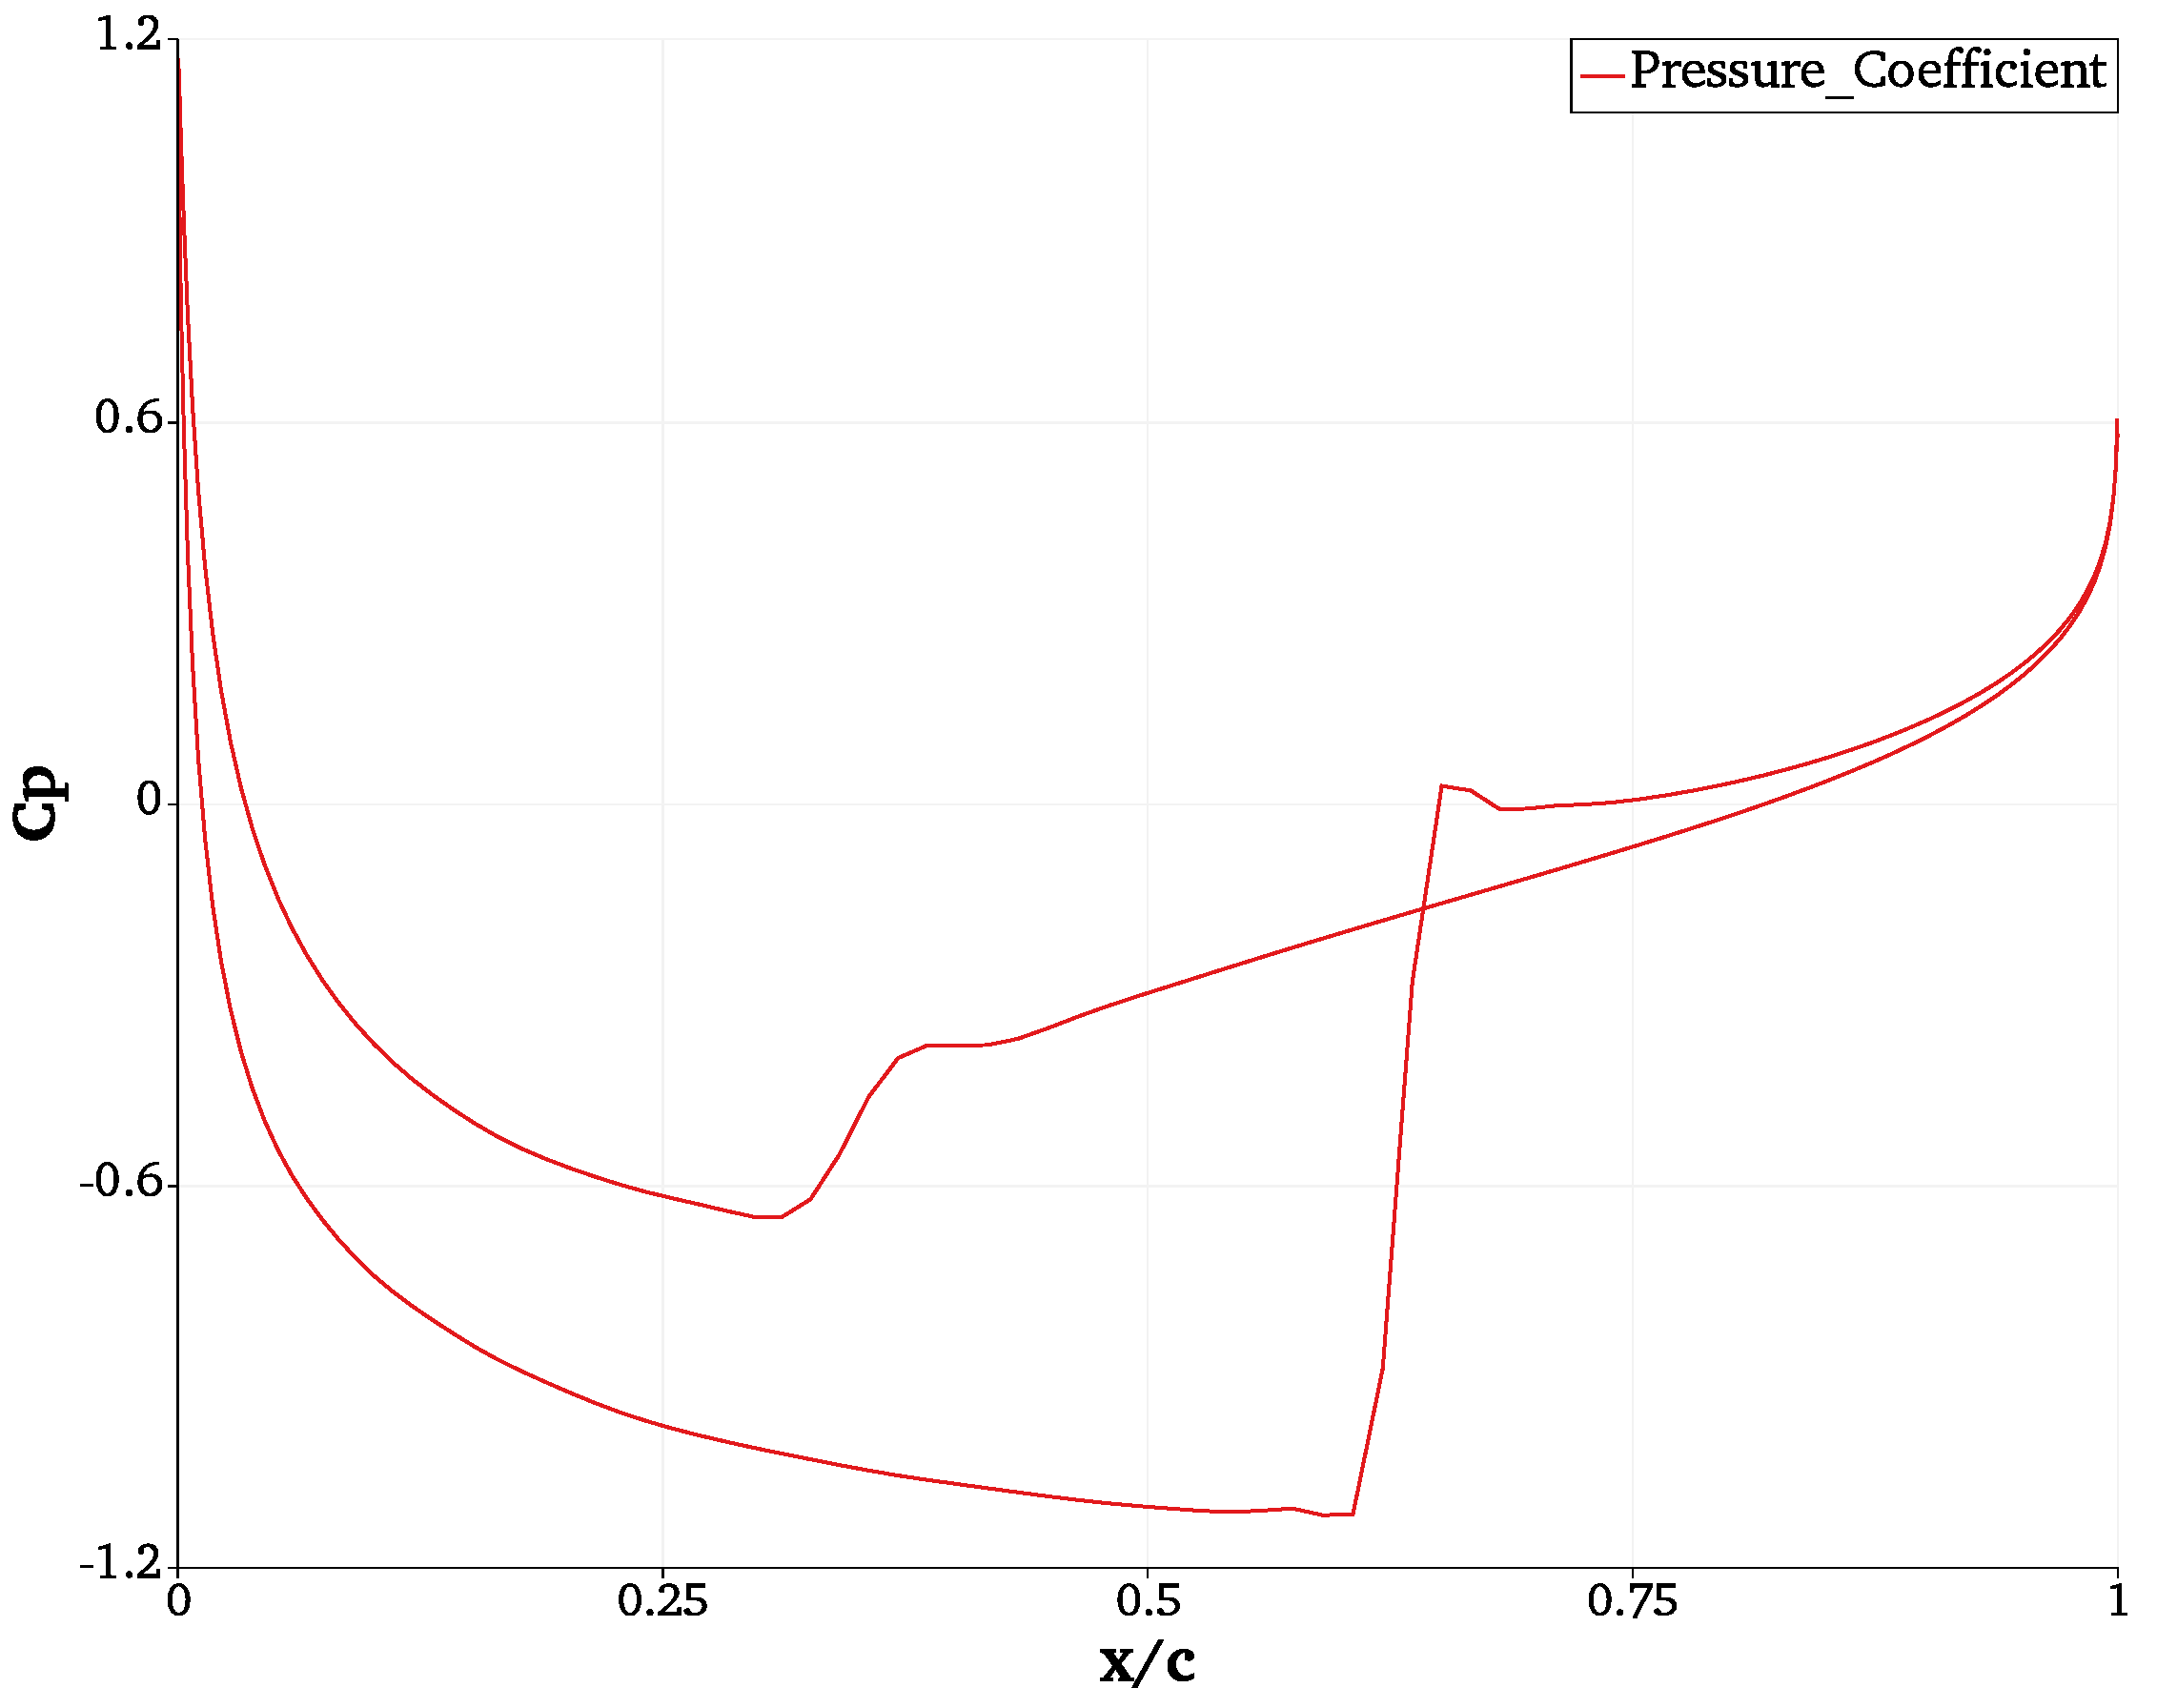
\includegraphics[width=.75\textwidth]{tut01/plot11.pdf}
    \caption{Pressure coefficient on the surface of the NACA0012.}
    \label{fig:surface_pressure}
\end{figure}

Usually $C_p$ is plotted in such a way that the pressure curve in suction side (lower pressure) is on top of the pressure curve on the pressure side (higher pressure). Therefore, we need to reverse  the $y$-axis in the plot (flip). To do this, go to \textbf{Display} from \textbf{Properties} tab. Next, find \textbf{Left Axis Range} section in the same tab, and then click on the \textbf{Left Axis Use Custom Range} (Fig.\ref{fig:viewsetting}). Later, another section appears to select maximum/minimum ranges for left axis of plot. Eventually, just switch numbers in these two text bars. It allows the $y$-axis to be reverse (flipped) as we want it to be.
\begin{figure}[htbp]
    \centering
    \includegraphics[width=0.5\textwidth]{tut01/leftaxis.pdf}
    \caption{Plot Settings.}
    \label{fig:viewsetting}
\end{figure}
Additionally, there are other parameters that you might change in the same tab, like \textbf{Left Axis Title} or  \textbf{Bottom Axis Title}. To do this, please type $C_p$ and $x/c$ in \textbf{Left Axis Title} and \textbf{Bottom Axis Title}, respectively. Furthermore, for adding marker to the plot lines, form \textbf{Display} select \textbf{Marker Style} as \textit{Diamond} (Fig.\ref{fig:marker}). You can also change the thickness of plot line in the same tab.
\begin{figure}[htbp]
    \centering
    \includegraphics[width=0.4\textwidth]{tut01/addingmarker.pdf}
    \caption{How to add marker to plot.}
    \label{fig:marker}
\end{figure}
Eventually, the final plot you should get is like Fig.\ref{fig:surface_pressure2}
\begin{figure}[htbp]
    \centering
    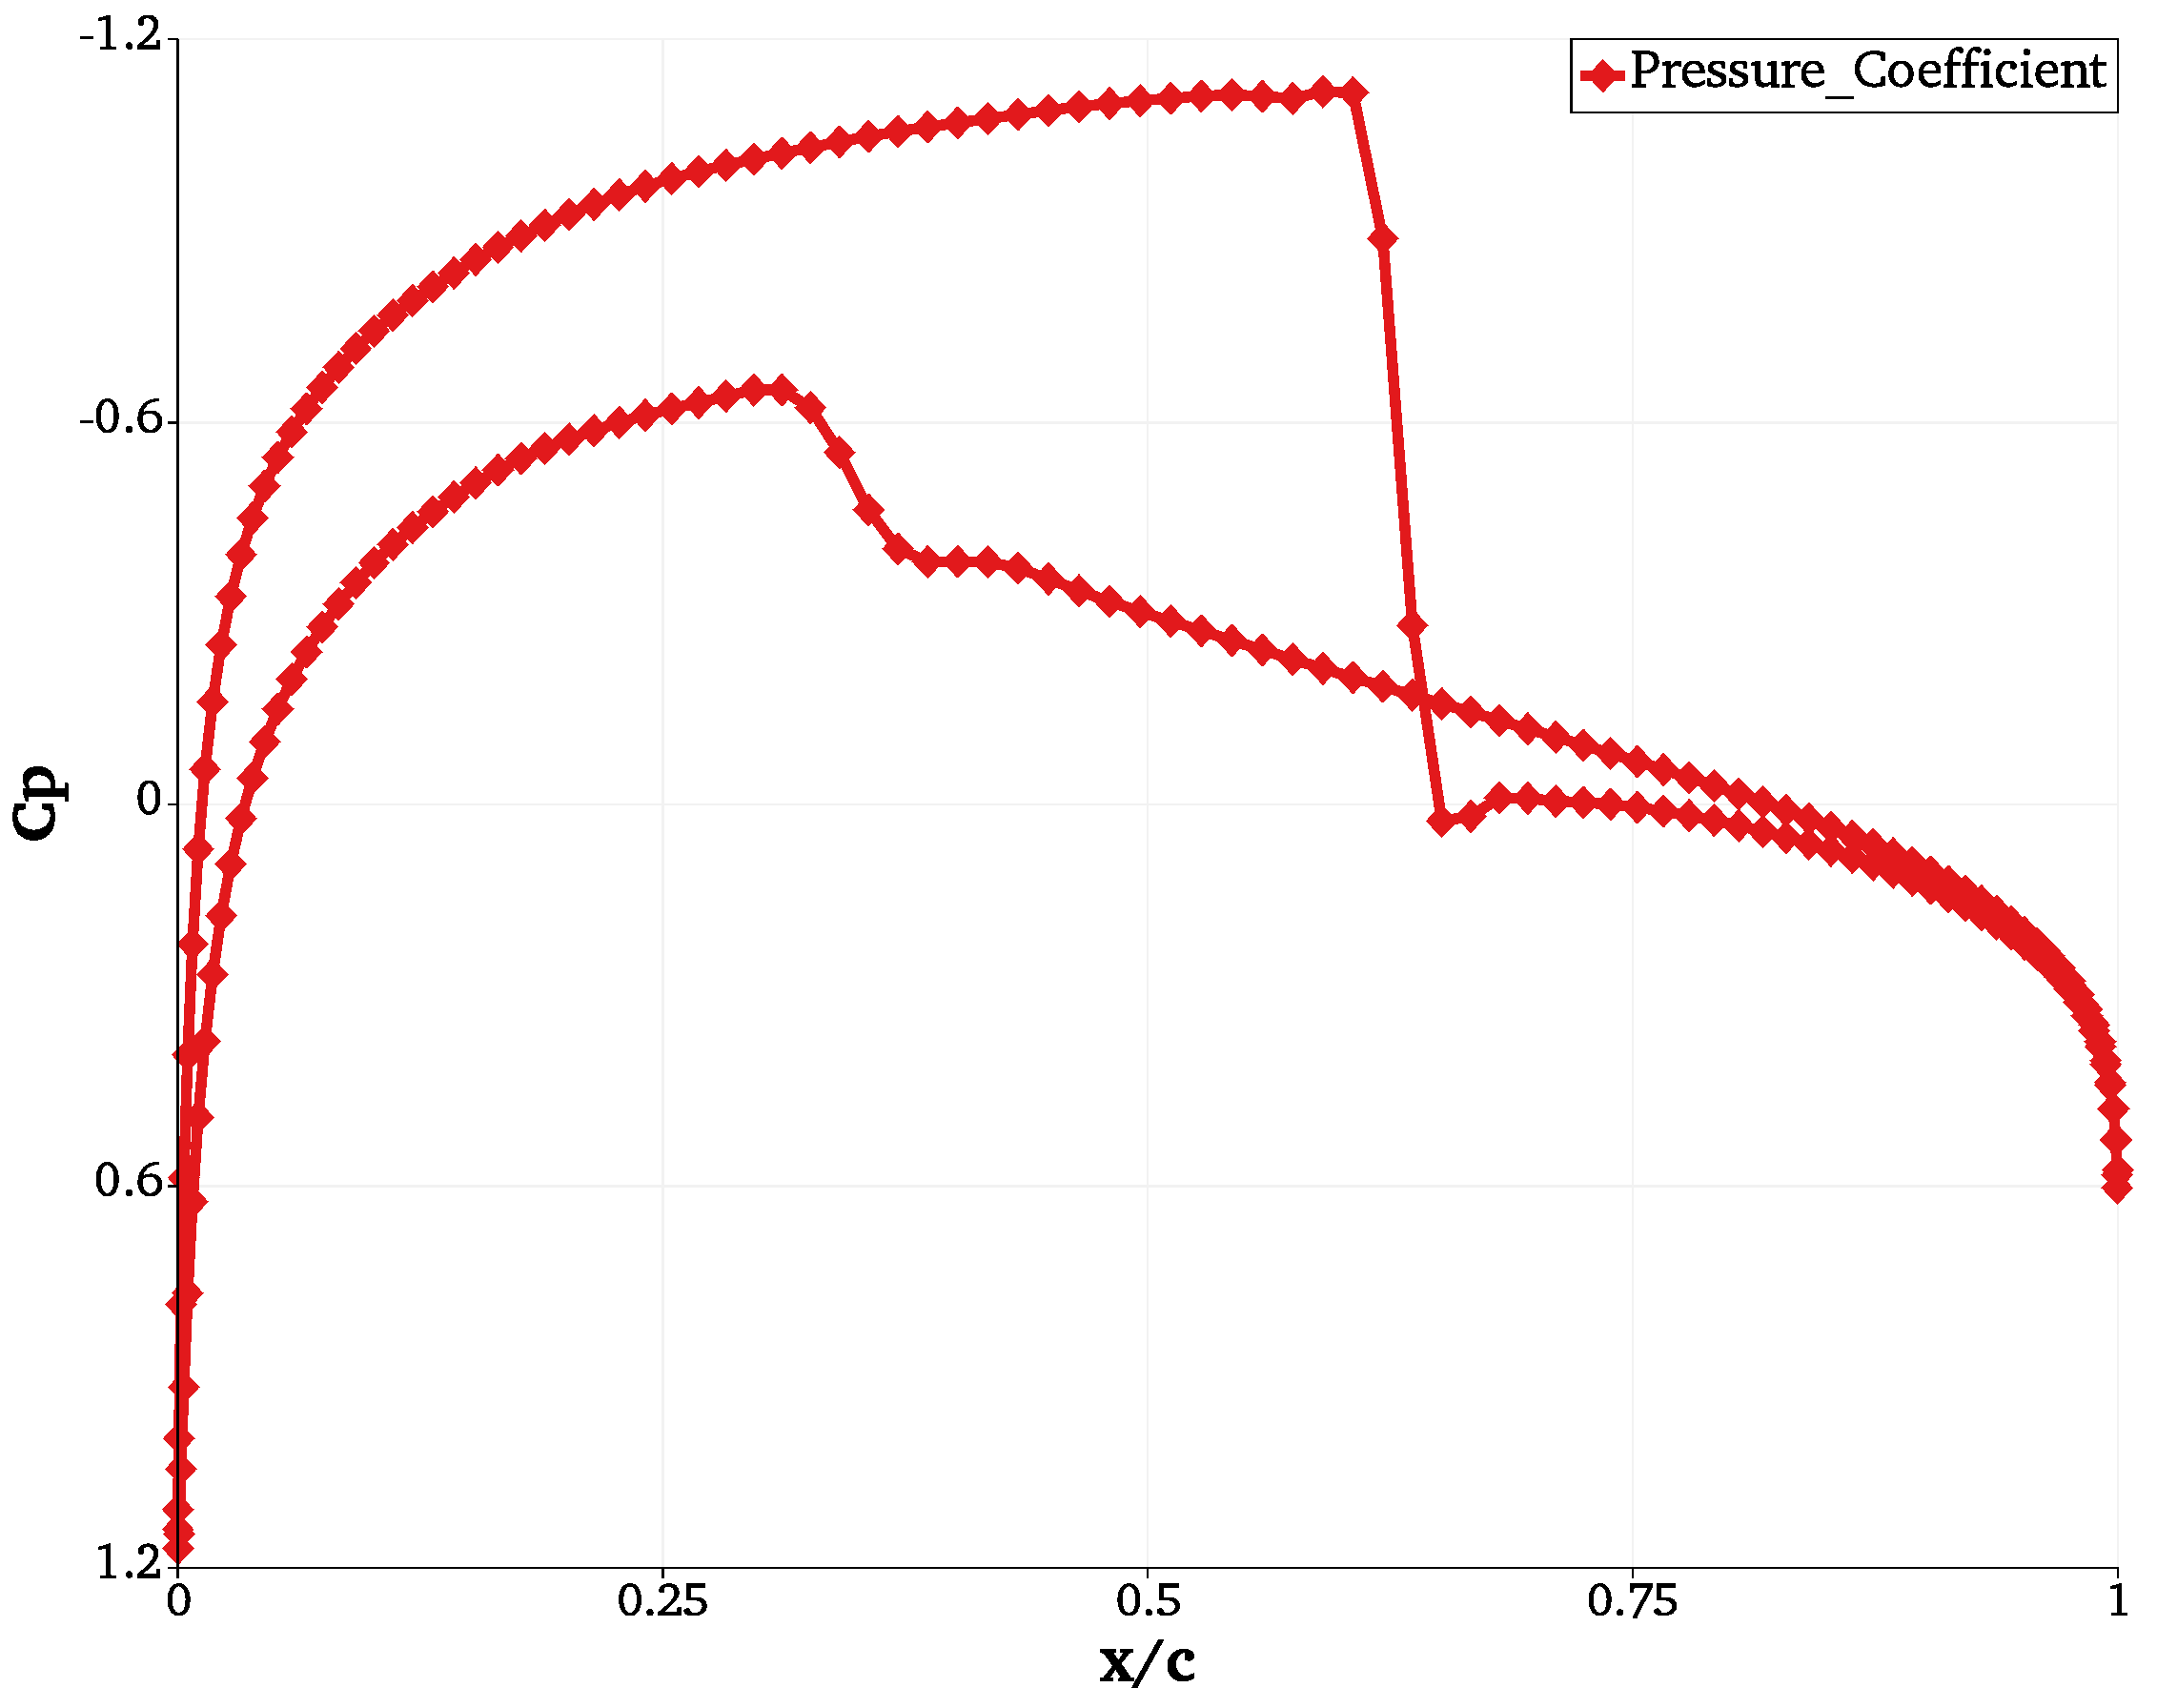
\includegraphics[width=.75\textwidth]{tut01/plot22.pdf}
    \caption{Revised version of the pressure coefficient plot on the surface of the NACA0012.}
    \label{fig:surface_pressure2}
\end{figure}
%--------------------------------------------------------------
\subsection{Forces on the Airfoil}
In order to obtain the aerodynamic loads on the airfoil, open \textit{force\_breakdown}.dat using a text editor software. According to Fig.\ref{fig:forcefile1}, in this file there are flow properties that you can check if the values are the same as those in configuration file. 
\begin{figure}[htbp]
    \centering
    \includegraphics[width=0.9\textwidth]{tut01/forcefile1.pdf}
    \caption{Fluid and flow properties form \textit{force\_breakdown}.dat.}
    \label{fig:forcefile1}
\end{figure}

Additionally, according to Fig.\ref{fig:forcefile2}, the aerodynamic loads are expressed in non-dimensional form by using free-stream values for density and velocity, as well as one reference length (or area). It could be a good practice to check if the non-dimensional factor corresponds to the expected free-stream values. The actual forces (dimensional) can be obtained by multiplying coefficient with non-dimensional factor calculated by free-stream density and velocity. Note that you can find lift coefficient ($C_L$), drag coefficient ($C_D$), lift to drag ratio ($C_L / C_D$), the moment coefficient ($C_{M,z}$), $x$-component of force coefficient ($C_{F,x}$) and $y$-component of force coefficient ($C_{F,y}$) all from the \textit{force\_breakdown}.dat.
\begin{figure}[htbp]
    \centering
    \includegraphics[width=0.8\textwidth]{tut01/forcefile2.pdf}
    \caption{Aerodynamic loads from \textit{force\_breakdown}.dat.}
    \label{fig:forcefile2}
\end{figure}
%++++++++++++++++++++++++++++++++++++++++++++++++++++++++++++++
\section{Questions}
1. Run the provided default NACA0012 test case at the provided Ma = 0.8.
\begin{enumerate}[label=(\alph*)]
    \item Plot and comment on the mesh.
    \item Plot and comment on the pressure contours around the airfoil.
    \item Plot and comment on the pressure coefficient on the surface of the airfoil.
\end{enumerate}
2. Re-run the default NACA0012 case but change the Mach number to Ma = 0.3 and run several simulations using alpha = 0, 2, 4, 6, 8, 10, 12, 14, 16 degrees.
\begin{enumerate}[label=(\alph*)]
    \item Plots Cl vs alpha alongside the provided experimental data \cite{ladson1988effects} in the test case folder.
    \item Repeat 1.b with Ma = 0.3 for the alpha = 0, 8, 16 degree cases.
    \item Repeat 1.c with for the alpha = 0, 8, 16 degree cases and include the provided experimental data  in the \cite{ladson1987pressure}.
\end{enumerate}
3. Compare your CFD results in Question 2). Discuss sources of error that could have led to any discrepancies in your results.
%--------------------------------------------------------------
%++++++++++++++++++++++++++++++++++++++++++++++++++++++++++++++
%++++++++++++++++++++++++++++++++++++++++++++++++++++++++++++++
%++++++++++++++++++++++++++++++++++++++++++++++++++++++++++++++
\chapter{Supersonic Wedge}
%++++++++++++++++++++++++++++++++++++++++++++++++++++++++++++++
\section{Problem Description}
In this tutorial, we are going to explain how to simulate supersonic inviscid flow past a simple 2D wedge. This wedge generates oblique-shock for high Mach number flows. Keep in mind that if the Reynolds number is high enough, the viscosity term in Navier-Stokes equations becomes negligible, and then, flow can be assumed to be inviscid. The another assumption we take is that the flow is a perfect gas. Furthermore, the domain is a structured mesh with 3,750 nodes. The upper wall is a flat Euler wall. The lower wall is also Euler wall with a wedge starting at $x/L=1/3$, where $L$ is the length of duct. Additionally, the wedge angle is 10 degree. For this example, the flow specifications are provided as follows:
\begin{itemize}
    \item Pressure = 101,325 Pa
    \item Temperature = 273.15 K
    \item Mach number = 2.0
    \item Wedge angle = 10 degrees
\end{itemize}
The tutorial has two parts: Flow Solution and Post-processing. In the first part, we explain how to manage prerequisite files and settings, and how to run the CFD simulation using SU2. In the second part, we explain how to use Paraview software to visualize data obtained form SU2.
%++++++++++++++++++++++++++++++++++++++++++++++++++++++++++++++
\section{Flow solution}
To run the simulation, the SU2 needs two essential files: configuration file (.cfg) and mesh file (.su2). In this example, the following files are located in \textit{02InviscidSupersonicWedge} folder:
\begin{enumerate}
    \item inv\_wedge\_HLLC.cfg as a configuration file.
    \item mesh\_wedge\_inv.su2 as a mesh file.
\end{enumerate}
The next step is to copy these two files in directory of SU2, where the execution and script files are located there. To run this simulation, open the command line terminal and enter the following commands:
\begin{table}[htbp]
    \centering
    \begin{tabular}{|l|l|}
    \hline
    Windows     & \begin{tabular}{c} \$ cd "where you saved the package" \\ \$ SU2\_CFD.exe inv\_wedge\_HLLC.cfg \end{tabular}
    \\
    \hline
    OSX     & \begin{tabular}{c} \$ cd "where you saved the package" \\ \$ SU2\_CFD.exe inv\_wedge\_HLLC.cfg \end{tabular}
    \\
    \hline
    \end{tabular}
\end{table}

The SU2 solver will commence calculation and print out the residuals at every iteration until the specified convergence criteria is achieved. After calculations are done, the following output files should be generated and saved in the SU2 folder:
\begin{itemize}
    \item \textit{flow}.vtk: contains the full volume flow solution.
    \item \textit{force\_breakdown}.dat: contains forces and moment on the surface of the duct.
    \item \textit{history}.vtk: contains convergence history of calculations.
    \item \textit{restart\_flow}.dat: for restarting simulation.
    \item \textit{surface\_flow}.vtk: flow solution on the surface of the duct.
    \item \textit{surface\_flow}.csv: comma separated values of flow solution on the surface of the duct (If you want to plot data in another software, like Microsoft Excel, you can use this file).
\end{itemize}
Please keep in mind that every time you run SU2, the output data will be overwritten. Hence, before launching new simulation, you could make a new folder and transfer your data from previous simulation to this folder.
%++++++++++++++++++++++++++++++++++++++++++++++++++++++++++++++
\section{Post-processing}
In this section, we explain how to use Paraview to visualize CFD data for this example. First of all, install Paraview (this tutorial uses Paraview 3.12.0) if you do not have it on your computer. Otherwise, take following steps for visualization:
%--------------------------------------------------------------
\subsection{Load Solution File:}
Launch Paraview. Go to \textbf{File} $\rightarrow$ \textbf{Open}, and then select \textit{flow}.vtk file. On the left side of Paraview window you will see the file appears in \textbf{Pipeline Browser}, under \textbf{builtin}. Now press \textbf{Apply} button in \textbf{Properties} tab, just right under the  \textbf{Pipeline Browser}. After taking these steps, your file is loaded by software and is ready to visualize (Fig.\ref{fig:load}).
\begin{figure}[htbp]
    \centering
    \includegraphics[width=0.4\textwidth]{tut02/loadvtkfile.pdf}
    \caption{Loading .vtk file in the \textbf{Pipeline Browser}.}
    \label{fig:load}
\end{figure}
%--------------------------------------------------------------
\subsection{Visualize Mesh Domain}
According to Fig.\ref{fig:wireframe}, in order to view mesh, select \textit{Solid Color} with \textit{Wireframe} in the toolbar. Then, you can even zoom in to see mesh for wedge domain, like Fig.\ref{fig:mesh}. As you can see, the mesh in the duct is structured, and at some point the wedge changes the direction of mesh in domain. Additionally, the grids are approximately uniform in whole domain without any significant clustering.
\begin{figure}[htbp]
    \centering
    \includegraphics[width=0.6\textwidth]{tut02/wireframe.pdf}
    \caption{How to display mesh in computational domain.}
    \label{fig:wireframe}
\end{figure}
\begin{figure}[htbp]
    \centering
    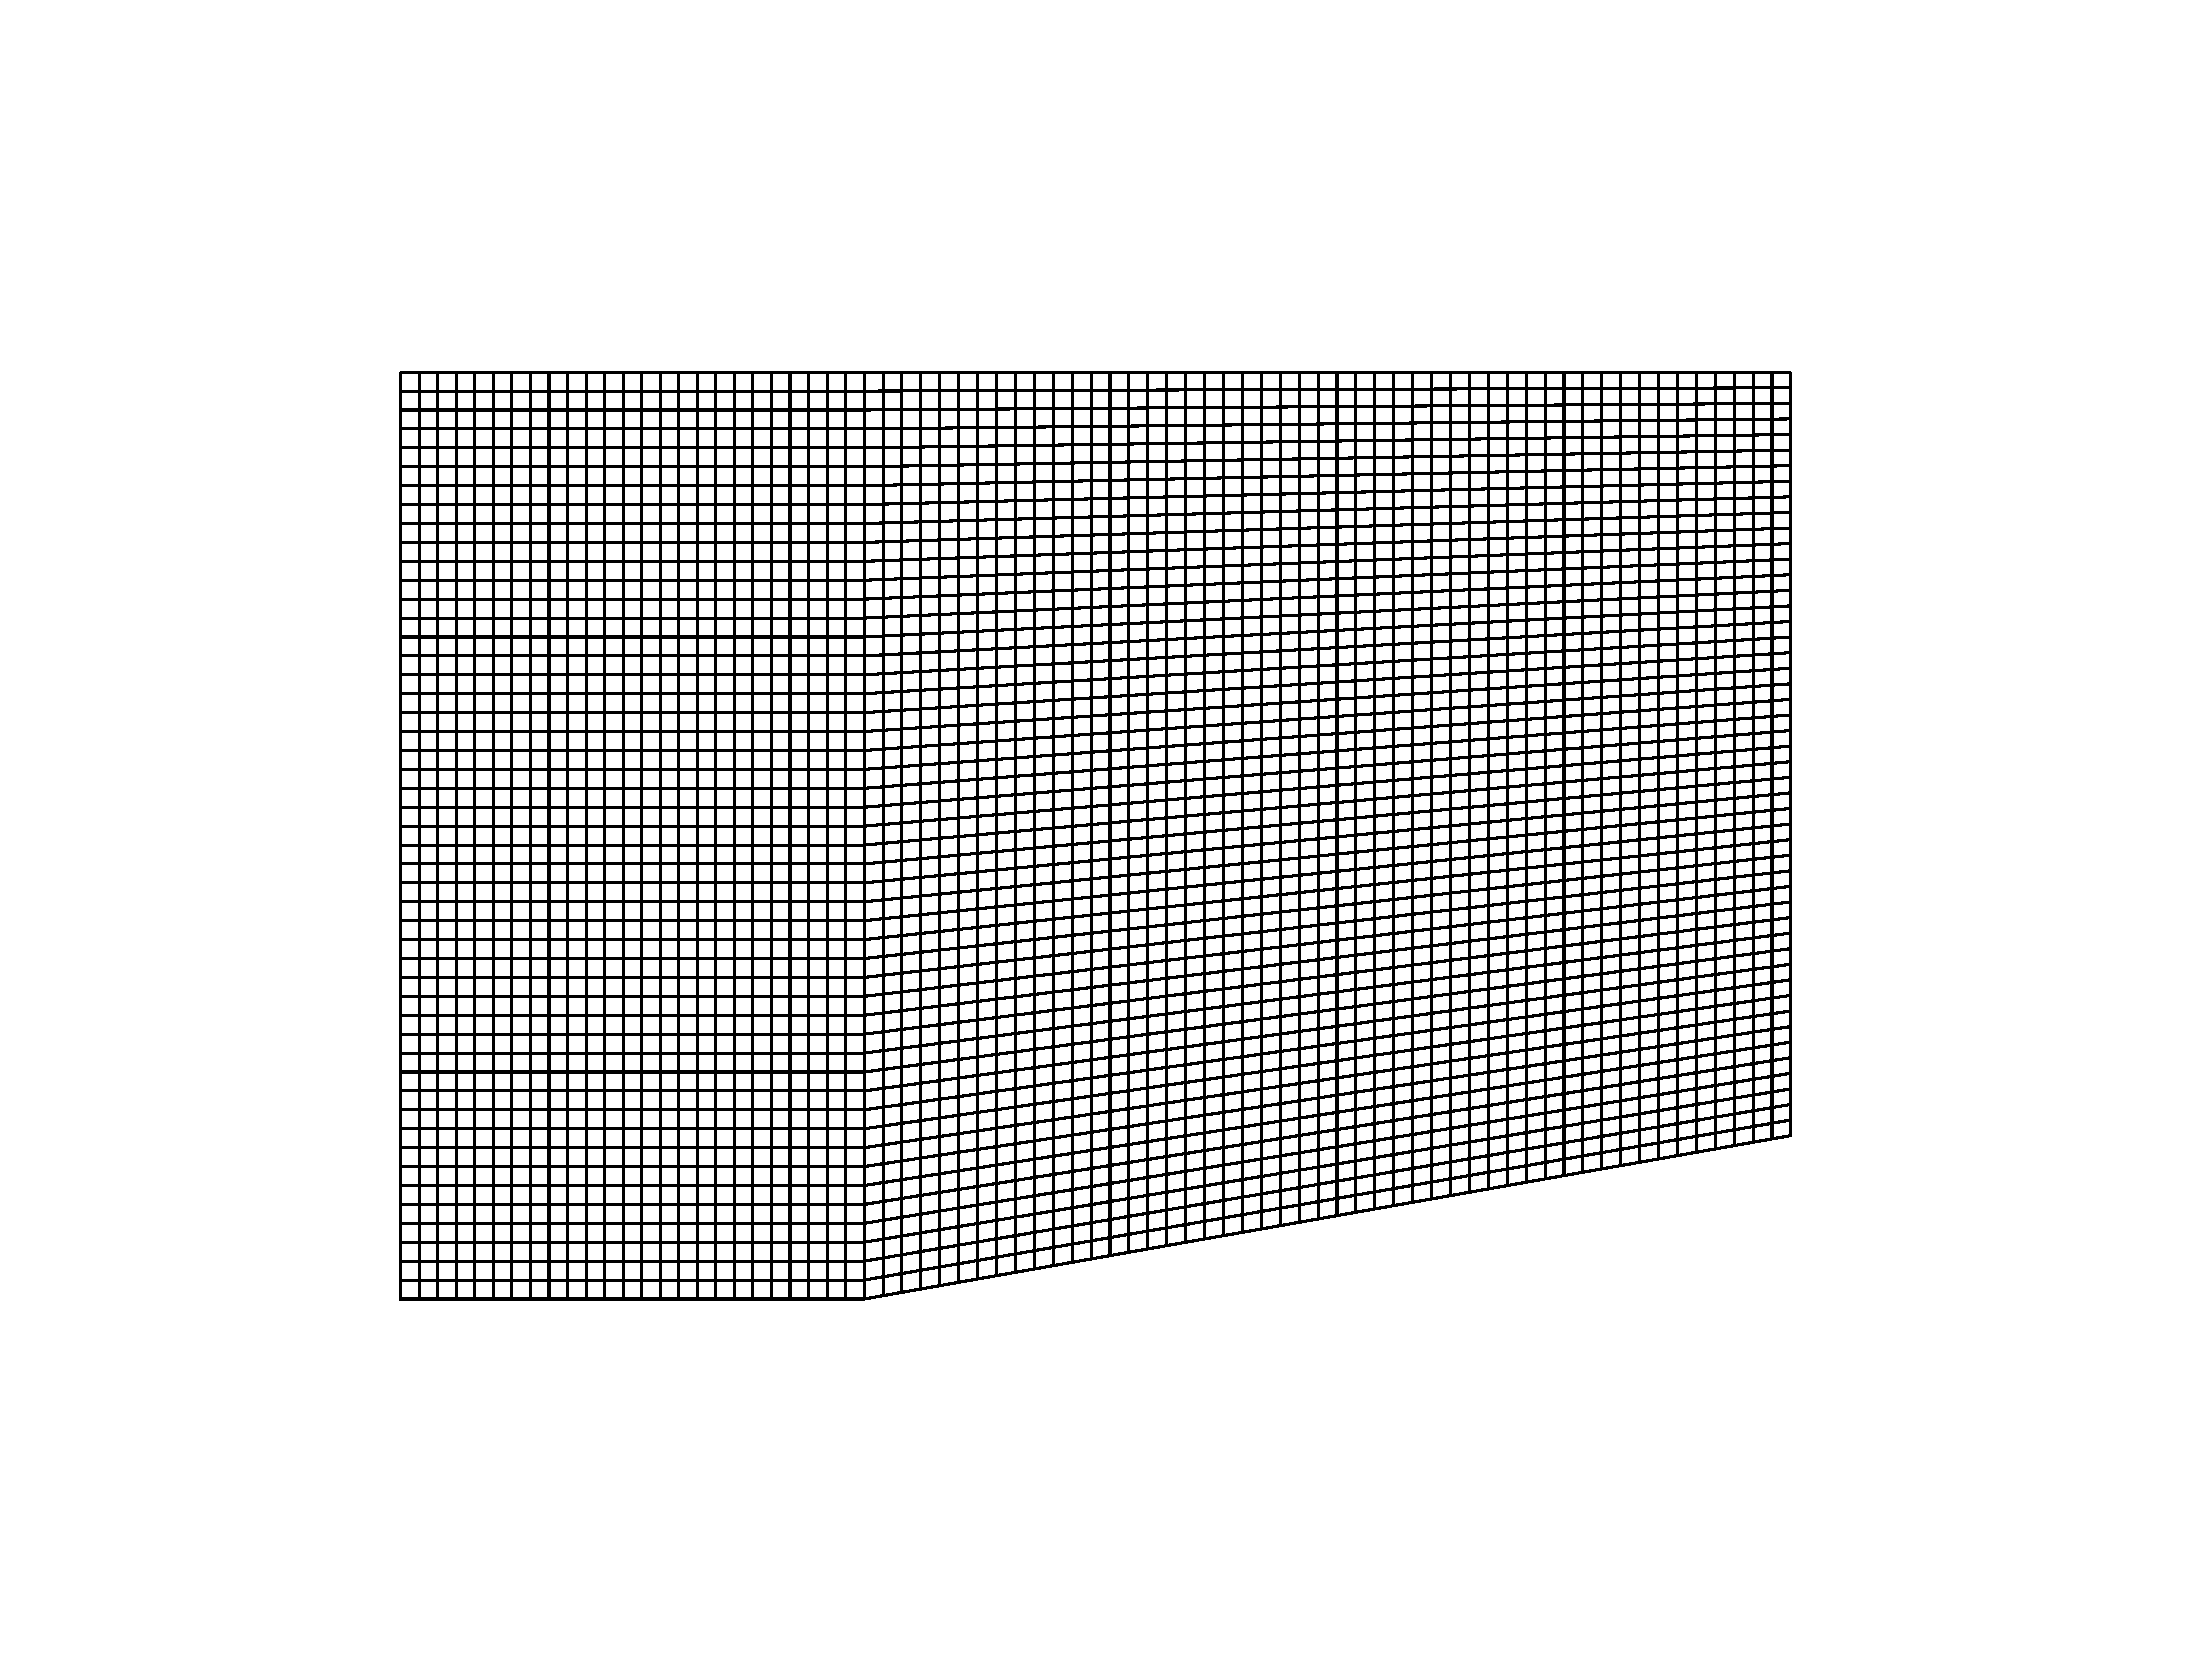
\includegraphics[width=.75\textwidth]{tut02/mesh.pdf}
    \caption{Structured mesh for wedge domain.}
    \label{fig:mesh}
\end{figure}
%--------------------------------------------------------------
\subsection{Visualize Pressure Contour and Mach Contour}
To display the pressure contour, click on the \textit{flow}.vtk in \textbf{Pipeline Browser} to activate the file, and then click on \textbf{Display} form \textbf{Properties} tab. Under \textbf{Coloring} section, select \textit{Pressure} from drop-down menu (Fig.\ref{fig:pressure contours setting}). Additionally, for changing color settings for the pressure, you can click on the \textbf{Edit} under the \textbf{Coloring}.
\begin{figure}[htbp]
    \centering
    \includegraphics[width=0.4\textwidth]{tut02/pressurecont.pdf}
    \caption{Settings for displaying the pressure contour.}
    \label{fig:pressure contours setting}
\end{figure}
Normally, another display window appears on the right-hand side of the monitor, named as \textbf{Mapping Data}, similar to Fig.\ref{fig:color_range}.
\begin{figure}[htbp]
    \centering
    \includegraphics[width=0.4\textwidth]{tut02/colorrange.pdf}
    \caption{Changing color range for pressure contour.}
    \label{fig:color_range}
\end{figure}
Now you can change contour colors by choosing \textbf{Choose preset}. Here, we select \textit{Cold and Hot} color range to be able to show clearly the sharp changes in pressure values (Fig.\ref{fig:color_range_item}). Then, click \textbf{Apply} for the next step.
\begin{figure}[htbp]
    \centering
    \includegraphics[width=0.5\textwidth]{tut02/changecontourcolors.pdf}
    \caption{Different color ranges to display contour.}
    \label{fig:color_range_item}
\end{figure}
Additionally, to add axis to plots, under \textbf{Miscellaneous} form \textbf{Display} (Fig.\ref{fig:add axis}), you can check box beside \textbf{Data Axes Grid}, and then go to \textbf{Edit} and change more options based on your preferences (Fig.\ref{fig:axis setting}).
\begin{figure}[htbp]
    \centering
    \includegraphics[width=0.4\textwidth]{tut02/addaxis.pdf}
    \caption{How to add axis to the plots.}
    \label{fig:add axis}
\end{figure}
\begin{figure}[htbp]
    \centering
    \includegraphics[width=0.6\textwidth]{tut02/axissettings.pdf}
    \caption{Settings for axis style.}
    \label{fig:axis setting}
\end{figure}
Finally, the pressure contour you get should be similar to Fig.\ref{fig:plot pressure cont1}.
\begin{figure}[htbp]
    \centering
    \includegraphics[width=0.85\textwidth]{tut02/plot1pressurecont.pdf}
    \caption{Pressure contour for supersonic wedge.}
    \label{fig:plot pressure cont1}
\end{figure}
%----------------------------------------------------------

The pressure gradient along the shock wave is very difficult to see, and we want to add contour lines to
separate the pressure color gradient. To add contour lines, click again on the \textit{flow}.vtk file in the \textbf{Pipeline Browser}, and then click on the \textbf{Contour} icon (Fig.\ref{fig:contour_icon}) in toolbar.
\begin{figure}[htbp]
    \centering
    \includegraphics[width=0.5\textwidth]{tut02/contourlineicon.pdf}
    \caption{\textbf{Contour} icon in toolbar.}
    \label{fig:contour_icon}
\end{figure}
Eventually,\textit{Contour1} appears under \textit{flow}.vtk file in the \textbf{Pipeline Browser} (Fig.\ref{fig:contour1}). Then, click on \textbf{Apply} to proceed next step.
\begin{figure}[htbp]
    \centering
    \includegraphics[width=0.4\textwidth]{tut02/contour1.pdf}
    \caption{Adding \textit{Contour1} in \textbf{Pipeline Browser}.}
    \label{fig:contour1}
\end{figure}
With regard to Fig.\ref{fig:contourby a}, go to the \textbf{Properties} tab, and select \textit{Pressure} from \textbf{Contour By} drop-down menu. Next, click on the \textbf{Add Range} icon to customize the range of pressure contour. In Fig.\ref{fig:contourby b}, you will see the max/min range of contour lines (i.e. \textbf{From}/\textbf{To}), as well as number of lines you would rather to have in your contour plot (i.e. \textbf{Steps}). Next, set \textbf{Step} to 20, and click \textbf{OK}. By doing this, it means the pressure contour range is equally divided by 20 portions, and the pressure values in each portion are limited by two lines in the display window. At the end, click on \textbf{Apply} to see contour lines in display window.
\begin{figure}[htbp]
    \centering
     \begin{subfigure}[b]{.4\textwidth}
         \centering
         \includegraphics[width=1.0\textwidth]{tut02/contourby.pdf}
         \caption{Define new range}
         \label{fig:contourby a}
     \end{subfigure}
     \hfill
     \begin{subfigure}[b]{.4\textwidth}
         \centering
         \includegraphics[width=1.0\textwidth]{tut02/addrange.pdf}
         \caption{Add range}
         \label{fig:contourby b}
     \end{subfigure}     
    \caption{How to define a new range for the contour lines.}
    \label{fig:contourby}
\end{figure}
Next, as it is shown in Fig.\ref{fig:colorby2}, click on the \textbf{Display} under \textbf{Properties} tab. In \textbf{Coloring} section, select \textbf{Solid Color} form drop-down menu, and choose white color form \textbf{Edit}.
\begin{figure}[htbp]
    \centering
    \includegraphics[width=0.4\textwidth]{tut02/contourline.pdf}
    \caption{Changing contour lines color in \textbf{Coloring} section.}
    \label{fig:colorby2}
\end{figure}
Eventually, the pressure contour with contour lines should be similar to Fig.\ref{fig:pressure_contour_lines}.
\begin{figure}[htbp]
    \centering
    \includegraphics[width=.85\textwidth]{tut02/plot2pressurecont.pdf}
    \caption{Pressure contour superimposed by contour lines for supersonic wedge.}
    \label{fig:pressure_contour_lines}
\end{figure}
You can zoom-in to the region at the bottom of the wedge to see the pressure gradient along the oblique
shock, like Fig.\ref{fig:pressure_contour_lines_zoom}.
\begin{figure}[htbp]
    \centering
    \includegraphics[width=.65\textwidth]{tut02/plot3pressurecont.pdf}
    \caption{Magnified pressure contour superimposed by contour lines for supersonic wedge.}
    \label{fig:pressure_contour_lines_zoom}
\end{figure}

The other important plot we want to show is related to Mach number contour. To display the Mach number contour, click on \textit{flow}.vtk in the \textbf{Pipeline Browser}. Similar to Fig.\ref{fig:pressure contours setting}, under \textbf{Coloring} section, select \textit{Mach} from drop-down menu. Next, click on \textit{Contour1} in the \textbf{Pipeline Browser}. Later, under \textbf{Properties}, select \textit{Mach} from \textbf{Contour By} drop-down menu. Since all the settings are related to pressure value, we need to revise some options for \textit{Mach} value. To do this, first of all, we need to delete data range for pressure and replace it with data range of Mach number. Under \textbf{Isosurfaces} from \textbf{Properties}, click on the \textbf{Remove All} icon, and then click on the \textbf{Add Range} icon, as shown in Fig.\ref{fig:contourby2 a}. As you can see form Fig.\ref{fig:contourby2 b}, the max/min values for mach number has changed. Now set the \textbf{Steps} to 20 and click on \textbf{OK} to proceed next step.
\begin{figure}[htbp]
    \centering
     \begin{subfigure}[b]{.4\textwidth}
         \centering
         \includegraphics[width=1.0\textwidth]{tut02/deladdrange.pdf}
         \caption{Define new range}
         \label{fig:contourby2 a}
     \end{subfigure}
     \hfill
     \begin{subfigure}[b]{.4\textwidth}
         \centering
         \includegraphics[width=1.0\textwidth]{tut02/addrange2.pdf}
         \caption{Add range}
         \label{fig:contourby2 b}
     \end{subfigure}     
    \caption{How to define a new range for the contour lines.}
    \label{fig:contourby2}
\end{figure}
Now the Mach number contour should look like Fig.\ref{fig:mach_contour}. Additionally, if you zoom-in the plot, you will see more contour details near the wedge similar to Fig.\ref{fig:mach_contour_zoom}.
\begin{figure}[htbp]
    \centering
    \includegraphics[width=.85\textwidth]{tut02/plot1machcont.pdf}
    \caption{Mach number contour superimposed by contour lines for supersonic wedge.}
    \label{fig:mach_contour}
\end{figure}
\begin{figure}[htbp]
    \centering
    \includegraphics[width=.65\textwidth]{tut02/plot1machcont2.pdf}
    \caption{Magnified Mach number contour superimposed by contour lines for supersonic wedge.}
    \label{fig:mach_contour_zoom}
\end{figure}
%--------------------------------------------------------------
\subsection{Plotting a variable over an arbitrary line}
For plotting variable over an arbitrary line, you can activate \textit{flow}.vtk by clicking on it in the \textbf{Pipeline Browser}. Next, as shown in Fig.\ref{fig:plot_over_line}, go to \textbf{Filters} $\rightarrow$  \textbf{Data Analysis} $\rightarrow$  \textbf{Plot Over Line}.
\begin{figure}[htbp]
    \centering
    \includegraphics[width=.75\textwidth]{tut02/plotoverline.pdf}
    \caption{How to plot over an arbitrary line.}
    \label{fig:plot_over_line}
\end{figure}
Next, according to Fig.\ref{fig:line_coordinate}, under \textbf{Line Parameters} from \textbf{Properties}, select the coordinates for two arbitrary points you want (i.e. \textbf{Point1} and \textbf{Point2}). In this case, plot the line from \textbf{Point1} to \textbf{Point2} with (0,0.5,0) and (1.5,0.5,0), respectively, and then, click on \textbf{Apply}.
\begin{figure}[htbp]
    \centering
    \includegraphics[width=.45\textwidth]{tut02/linecoord.pdf}
    \caption{Define the coordinates for plotting over the line.}
    \label{fig:line_coordinate}
\end{figure}
Eventually, a plot will be generated. According to Fig.\ref{fig:plot_line_setting}, under \textbf{X Axis Parameters} from \textbf{Display}, pick \textit{Point\_X} from \textbf{X Array Name} drop-down menu. Furthermore, under \textbf{Series Parameters}, toggle the box beside \textbf{Variable} to uncheck everything, then select the \textit{Mach} among all variables existed.
\begin{figure}[htbp]
    \centering
    \includegraphics[width=.45\textwidth]{tut02/plotmachline.pdf}
    \caption{How to plot Mach number over a line.}
    \label{fig:plot_line_setting}
\end{figure}
The plot of Mach number vs the \textit{x-coordinate} will be displayed in main window like Fig.\ref{fig:plot_line}.
\begin{figure}[htbp]
    \centering
    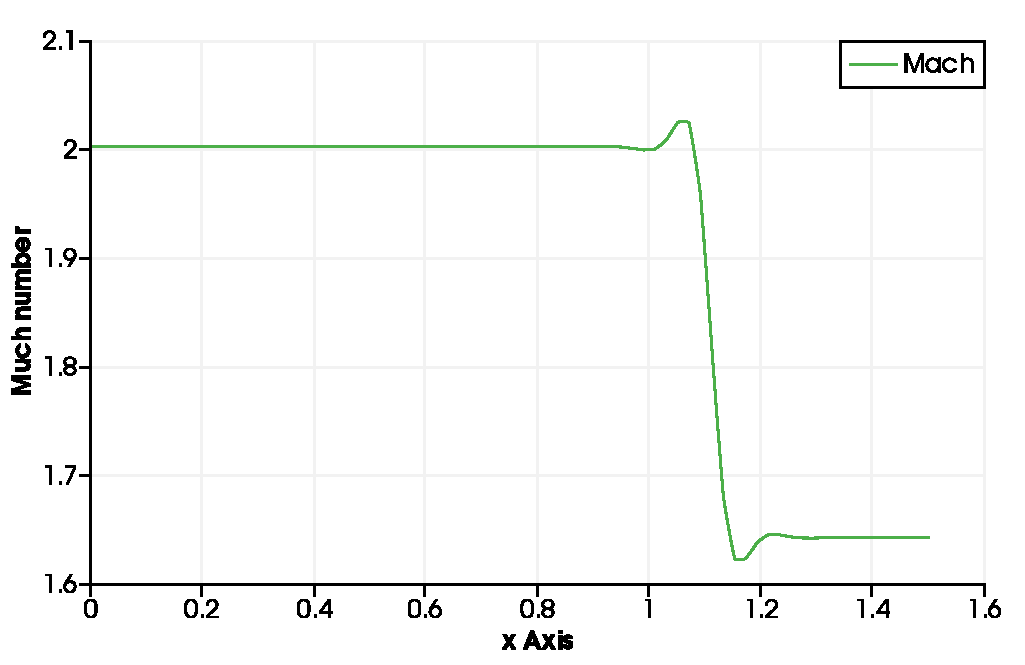
\includegraphics[width=.85\textwidth]{tut02/plot2contourline.pdf}
    \caption{Mach number plot over a specified line in \textit{x-coordinate}.}
    \label{fig:plot_line}
\end{figure}
In order to see the spreadsheet view, click the upper right icon as shown in Fig.\ref{fig:open_spreadsheet}, then click on the \textit{Spreadsheet View} like Fig.\ref{fig:spreadsheet}.
\begin{figure}[htbp]
    \centering
    \includegraphics[width=.3\textwidth]{tut02/openspreadsheet.pdf}
    \caption{How to make spreadsheet view in a new window.}
    \label{fig:open_spreadsheet}
\end{figure}
\begin{figure}[htbp]
    \centering
    \includegraphics[width=.65\textwidth]{tut02/spreadsheet.pdf}
    \caption{Selecting \textit{Spreadsheet View} among different views.}
    \label{fig:spreadsheet}
\end{figure}
Additionally, you can save .csv file and plot it with other available software such as Microsoft Excel. To export the spreadsheet as a .csv file, go to \textbf{File} $\rightarrow$ \textbf{Export}, and then \textbf{Save as} .csv.
%++++++++++++++++++++++++++++++++++++++++++++++++++++++++++++++
\section{Questions}
1. Run the default case as provided which uses 2ND\_ORDER and the HLLC Riemann solver.
\begin{enumerate}[label=(\alph*)]
    \item Create coloured contours of Pressure and Mach number in the entire domain.
    \item Plot Pressure from (0,0.5,0) to (1.5,0.5,0) using the \textbf{Plot Over Line}.
\end{enumerate}
2. Repeat Q.1 but switch the SPATIAL\_ORDER\_FLOW to 1ST\_ORDERs. \\
3. Repeat 1 using SPATIAL\_ORDER\_FLOW as 2ND\_ORDER but using the JST flux. \\
4. Repeat Q.1 using SPATIAL\_ORDER\_FLOW as 2ND\_ORDER but using the LAX-FRIEDRICH flux. \\
5. Repeat Q.1 using SPATIAL\_ORDER\_FLOW as 2ND\_ORDER but using the CUSP flux. \\
6. Repeat Q.1 using SPATIAL\_ORDER\_FLOW as 2ND\_ORDER but using the ROE flux. \\
7. Comment on how spatial order of accuracy and choice of Riemann solver affects the resolution of the shock and any dissipation or dispersion errors you can observe.
%++++++++++++++++++++++++++++++++++++++++++++++++++++++++++++++
%++++++++++++++++++++++++++++++++++++++++++++++++++++++++++++++
%++++++++++++++++++++++++++++++++++++++++++++++++++++++++++++++
\chapter{Inviscid ONERA M6}
%++++++++++++++++++++++++++++++++++++++++++++++++++++++++++++++
\section{Problem Description}
In this tutorial, we are going to explain how to simulate external, compressible, and transonic inviscid flow past a 3D wing. The chosen wing is ONERA M6 which is a well-known CFD test case for supersonic flows. This wing was designed by ONERA Aerodynamics Department as a bench mark for experimental studies. Due to availability of experimental data and simple geometry of wing, this wing has also attracted the attention of CFD engineers. Furthermore, CFD analysis of ONERA M6 wing is notable, since some of important phenomena occurs in this case, like transonic-shock, flow separation over the wing, 3D structure of flow around the tip of the wing. In this tutorial, the computational domain with unstructured mesh consists of 582,752 tetrahedral elements and 108,396 nodes. For this example, the flow specifications are provided as follows:
\begin{itemize}
    \item Pressure = 101,325 Pa
    \item Temperature = 273.15 K
    \item Mach number = 0.8395
    \item angle of attack = 3.06 degrees
\end{itemize}

The tutorial has two parts: Flow Solution and Post-processing. In the first part, we explain how to manage prerequisite files and settings, and how to run the CFD simulation using SU2. In the second part, we explain how to use Paraview software to visualize data obtained form SU2.
%++++++++++++++++++++++++++++++++++++++++++++++++++++++++++++++
\section{Flow solution}
In the configuration file, you can specify the multi-grid parameters. For the tutorial case, you will see that \texttt{MGLEVEL=0}. However, you can choose different level for your multi-grid method by giving an integer number to \texttt{MGLEVEL}. You can also select type of multi-grid cycle by setting one of existing options in \texttt{MGCYCLE (V Cycle, W Cycle or Full MG Cycle)}. Another parameter of interest is the total number of iterations. This can be modified by changing the value in \texttt{EXT\_ITER}. For this example it will be kept at 200 for brevity; but depending on the method used, higher iteration numbers may be necessary before solution can converge. In this tutorial, we want to look at the pressure coefficient and Mach number contours, solve for the lift coefficient ($C_L$) and drag coefficient ($C_D$) of the ONERA M6 wing, as well as observe the rate of convergence. This helps you to get to know how to speed up your simulation using multi-grid technique, and how to check convergence rate to assure your results are converged.

To run the simulation, the SU2 needs two essential files: configuration file (.cfg) and mesh file (.su2). In this example, the following files are located in \textit{03InviscidOneraM6} folder:
\begin{enumerate}
\item \textit{inv\_ONERAM6}.cfg as a configuration file.
\item \textit{mesh\_ONERAM6\_inv}.su2 as a mesh file.
\end{enumerate}
The next step is to copy these two files in directory of SU2, where the execution and script files are located there. To run this simulation, open the command line terminal and enter the following commands:
\begin{table}[htbp]
    \centering
    \begin{tabular}{|l|l|}
    \hline
    Windows     & \begin{tabular}{c} \$ cd "where you saved the package" \\ \$ SU2\_CFD.exe inv\_ONERAM6.cfg \end{tabular}
    \\
    \hline
    OSX     & \begin{tabular}{c} \$ cd "where you saved the package" \\ \$ SU2\_CFD.exe inv\_ONERAM6.cfg \end{tabular}
    \\
    \hline
    \end{tabular}
\end{table}

The SU2 solver will commence calculation and print out the residuals at every iteration until the specified convergence criteria is achieved. After calculations are done, the following output files should be generated and saved in the SU2 folder:
\begin{itemize}
    \item \textit{flow}.vtk: contains the full volume flow solution.
    \item \textit{force\_breakdown}.dat: contains forces and moment on the surface of the wing.
    \item \textit{history}.vtk: contains convergence history of calculations.
    \item \textit{restart\_flow}.dat: for restarting simulation.
    \item \textit{surface\_flow}.vtk: flow solution on the surface of the wing.
    \item \textit{surface\_flow}.csv: comma separated values of flow solution on the surface of the wing (If you want to plot data in another software, like Microsoft Excel, you can use this file).
\end{itemize}
Please keep in mind that every time you run SU2, the output data will be overwritten. Hence, before launching new simulation, you could make a new folder and transfer your data from previous simulation to this folder.
%++++++++++++++++++++++++++++++++++++++++++++++++++++++++++++++
\section{Post-processing}
In this section, we explain how to use Paraview to visualize CFD data for this example. First of all, install Paraview (this tutorial uses Paraview 3.12.0) if you do not have it on your computer. Otherwise, take following steps for visualization:
%--------------------------------------------------------------
\subsection{Load Solution File:}
Launch Paraview. Go to \textbf{File} $\rightarrow$ \textbf{Open}, and then select \textit{surface\_flow}.vtk file. On the left-hand side of Paraview window you will see the file appears under \textbf{builtin} in \textbf{Pipeline Browser}. Now press \textbf{Apply} button in \textbf{Properties} tab, just right under the  \textbf{Pipeline Browser}. After taking these steps, your file is loaded by software and is ready to visualize (Fig.\ref{fig:load}).
\begin{figure}[htbp]
    \centering
    \includegraphics[width=0.4\textwidth]{tut03/surface_flow.pdf}
    \caption{Loading \textit{surface\_flow}.vtk file in the \textbf{Pipeline Browser}.}
    \label{fig:load}
\end{figure}
%--------------------------------------------------------------
\subsection{Visualize Mesh Domain}
In order to view mesh, according to Fig.\ref{fig:wireframe}, select \textit{Solid Color} with \textit{Wireframe} in the toolbar. As you can see from Fig.\ref{fig:mesh}, the mesh around the ONERA M6 wing is unstructured, and the grids are clustered around the tip, leading and trailing edges of the wing. The reason for this clustering is that the changes in flow variables are high at these regions and the mesh should be fine enough at vicinity of these regions in order to solve flow accurately.
\begin{figure}[htbp]
    \centering
    \includegraphics[width=0.6\textwidth]{tut03/wireframe.pdf}
    \caption{How to display mesh in computational domain.}
    \label{fig:wireframe}
\end{figure}
\begin{figure}[htbp]
    \centering
    \includegraphics[width=.75\textwidth]{tut03/mesh2.pdf}
    \caption{Unstructured mesh around ONERA M6 wing.}
    \label{fig:mesh}
\end{figure}
%--------------------------------------------------------------
\subsection{Visualize Pressure Coefficient Contour and Much Number Contour}
To display the pressure contour, click on the \textit{surface\_flow}.vtk in the \textbf{Pipeline Browser}, and then click on the \textbf{Display} in \textbf{Properties} tab. Next, under \textbf{Coloring}, select \textit{Pressure\_Coefficient} from drop-down menu (Fig.\ref{fig:pressure_coeff_1}).
\begin{figure}[htbp]
    \centering
    \includegraphics[width=0.4\textwidth]{tut03/coloring.pdf}
    \caption{Display contour by selecting variable.}
    \label{fig:pressure_coeff_1}
\end{figure}
Eventually, the pressure coefficient contour should be similar to Fig.\ref{fig:plot_pressure_coeff}
\begin{figure}[htbp]
    \centering
    \includegraphics[width=0.65\textwidth]{tut03/cont1_pressure_coefficient.pdf}
    \caption{Pressure coefficient contour for ONERA M6 wing.}
    \label{fig:plot_pressure_coeff}
\end{figure}

In order to add contour lines to the plot, click again on the \textit{surface\_flow}.vtk in the \textbf{Pipeline Browser}, and then click on the \textbf{Contour} icon (Fig.\ref{fig:contour_icon}) in toolbar.
\begin{figure}[htbp]
    \centering
    \includegraphics[width=0.5\textwidth]{tut03/contourlineicon.pdf}
    \caption{\textbf{Contour} icon in toolbar.}
    \label{fig:contour_icon}
\end{figure}
Eventually, \textit{Contour1} appears under \textit{flow}.vtk file in the \textbf{Pipeline Browser} (Fig.\ref{fig:contour1}). Then, click on \textbf{Apply} to proceed next step.
\begin{figure}[htbp]
    \centering
    \includegraphics[width=0.4\textwidth]{tut03/contour1.pdf}
    \caption{Adding \textit{Contour1} in \textbf{Pipeline Browser}.}
    \label{fig:contour1}
\end{figure}
According to Fig.\ref{fig:contourby a}, go to the \textbf{Properties}, and choose \textit{Pressure\_Coefficient} from \textbf{Contour By} drop-down menu. Then, click on the \textbf{Add Range} icon to customize the range of pressure contour. As seen from Fig.\ref{fig:contourby b},  max/min (i.e. \textbf{From}/\textbf{To}) range of contour lines, as well as the number steps required to divide this range into the equal portions exist. So, set \textbf{Step} to 20, and click on \textbf{OK}. At the end, click on \textbf{Apply} to illustrate contour lines in display window.
\begin{figure}[htbp]
    \centering
     \begin{subfigure}[b]{.4\textwidth}
         \centering
         \includegraphics[width=1.0\textwidth]{tut03/pressure_coeff_addrange1.pdf}
         \caption{Define new range}
         \label{fig:contourby a}
     \end{subfigure}
     \hfill
     \begin{subfigure}[b]{.4\textwidth}
         \centering
         \includegraphics[width=1.0\textwidth]{tut03/pressure_coeff_addrange2.pdf}
         \caption{Add range}
         \label{fig:contourby b}
     \end{subfigure}     
    \caption{How to define a new range for the contour lines.}
    \label{fig:contourby}
\end{figure}
Next, as it is shown in Fig.\ref{fig:colorby2}, click on the \textbf{Display} under \textbf{Properties} tab. In \textbf{Coloring} section, select \textbf{Solid Color} form drop-down menu, and choose black color from \textbf{Edit}.
\begin{figure}[htbp]
    \centering
    \includegraphics[width=0.4\textwidth]{tut03/coloring2.pdf}
    \caption{Changing contour lines color in \textbf{Coloring} section.}
    \label{fig:colorby2}
\end{figure}
Eventually, the pressure contour with black contour lines should be similar to Fig.\ref{fig:pressure_contour_lines}.
\begin{figure}[htbp]
    \centering
    \includegraphics[width=.65\textwidth]{tut03/cont2_pressure_coefficient.pdf}
    \caption{Pressure coefficient contour superimposed by contour lines for ONERA M6 wing.}
    \label{fig:pressure_contour_lines}
\end{figure}

To display the Mach number contour, similar to Fig.\ref{fig:pressure_coeff_1}, click on the \textit{surface\_flow}.vtk in the \textbf{Pipeline Browser}, and under \textbf{Coloring} from \textbf{Display}, select \textit{Mach} from drop-down menu. In the next step, click on "\textit{Contour1}" in the \textbf{Pipeline Browser}. As it is shown in Fig.\ref{fig:contourby2 a}, under \textbf{Properties}, select \textit{Mach} from \textbf{Contour By} drop-down menu. Next, click on \textbf{Remove All} icon to remove previous value range belonged to pressure coefficient. Similar to Fig.\ref{fig:contourby2 b}, click on \textbf{Add Range} icon and set \textbf{Steps} to 20. Next, click on \textbf{OK}, and then, \textbf{Apply} to show plot.
\begin{figure}[htbp]
    \centering
     \begin{subfigure}[b]{.4\textwidth}
         \centering
         \includegraphics[width=1.0\textwidth]{tut03/del_add_range_mach.pdf}
         \caption{Define new range}
         \label{fig:contourby2 a}
     \end{subfigure}
     \hfill
     \begin{subfigure}[b]{.4\textwidth}
         \centering
         \includegraphics[width=1.0\textwidth]{tut03/AddRangemach.pdf}
         \caption{Add range}
         \label{fig:contourby2 b}
     \end{subfigure}     
    \caption{How to define a new range for the contour lines.}
    \label{fig:contourby2}
\end{figure}
Now the Mach number contour of the wing surface should be similar to Fig.\ref{fig:mach_contour}.
\begin{figure}[htbp]
    \centering
    \includegraphics[width=0.5\textwidth]{tut03/machcontour1.pdf}
    \caption{Mach number contour with superimposed by lines.}
    \label{fig:mach_contour}
\end{figure}
%--------------------------------------------------------------
\subsection{Comparison of Convergence Rate}
Launch Microsoft Excel or any other plotting software. For Microsoft Excel, open the file \textit{history}.vtk from the tutorial folder. Then, you are asked to choose the file type that best describes your data. You should select \textbf{Delimiters}, and in the next step, Under the \textbf{Delimiters}, select only the check boxes for \textit{Tab}, \textit{Semicolon}, and \textit{Comma} (Fig.\ref{Fig11}).
\begin{figure}[htbp]
    \centering
    \includegraphics[width=0.5\textwidth]{tut03/16.png}
    \caption{Import .vtk file in Microsoft Excel.}
    \label{Fig11}
\end{figure}
As shown in Fig.\ref{Fig12}, the first column shows the iteration number. The lift coefficient ($C_L$) and the drag coefficient ($C_D$) are displayed in the second and third column, respectively. Additionally, the residuals can also be examined to check convergence (Column \textit{L} to Column \textit{P} in Fig.\ref{Fig13}).
\begin{figure}[htbp]
    \centering
    \includegraphics[width=0.5\textwidth]{tut03/17.png}
    \caption{Columns in \textit{history}.vtk}
    \label{Fig12}
\end{figure}
\begin{figure}[htbp]
    \centering
    \includegraphics[width=0.75\textwidth]{tut03/18.png}
    \caption{Residuals in \textit{history}.vtk}
    \label{Fig13}
\end{figure}
Now we plot the lift coefficient, drag coefficient, and density residual against the number of iterations to see how many iterations it takes to converge to a steady solution. Fig.\ref{Fig14} and Fig.\ref{Fig15} shows the plots for aerodynamic loads and residual versus the number of iterations, respectively, for the case of \texttt{MGLEVEL=0} on tetrahedral mesh.
\begin{figure}[htbp]
    \centering
    \includegraphics[width=0.75\textwidth]{tut03/22.png}
    \caption{Lift and Drag coefficients versus the number of iterations.}
    \label{Fig14}
\end{figure}
\begin{figure}[htbp]
    \centering
    \includegraphics[width=0.75\textwidth]{tut03/21.png}
    \caption{Density residual versus the number of iterations.}
    \label{Fig15}
\end{figure}
%++++++++++++++++++++++++++++++++++++++++++++++++++++++++++++++
\section{Questions}
1. Run the simulation without multi-grid scheme (\texttt{MGLEVEL=0}).
\begin{enumerate}[label=(\alph*)]
    \item Follow the procedure in the guideline document to run the simulation and record the number of iterations and wall-clock time for the simulation to complete.
    \item Record the lift and drag coefficients.
    \item Plot the surface pressure coefficient with coloured contours and contour lines.
    \item Plot the surface Mach number with coloured contours and contour lines.
    \item Plot the value of $C_L$, $C_D$ and the density residual vs. the number of iterations.
\end{enumerate}
2. Modify the configuration file in the multi-grid folder (\texttt{MGLEVEL= 3, MGCYCLE= W\_CYCLE}) and repeat Q.1 using multi-grid scheme.\\
3. Compare the results in part (a)-(e) of Q.1 and Q.2. In what way is the use of multi-grid advantageous for this test case?\\
%++++++++++++++++++++++++++++++++++++++++++++++++++++++++++++++
\chapter{Laminar Cylinder}
\section{Problem Description}
In this tutorial, we are going to explain how to simulate the external flow past a 2D cylinder. To simulate viscous flow, Navier-Stokes equations are solved in steady or unsteady format, depending at Reynolds numbers. According to observations, the flow remains symmetric and steady for Reynolds number less than around 46, while at higher Reynolds number the flow becomes unstable and asymmetric. Therefore, in this time-dependent flow,  Von-Karman Streets appear, which is a well-known phenomenon in fluid mechanics. The Von-Karman Streets correspond to pair vortex shedding behind the cylinder, where vortices are generated due to flow unsteadiness and disturbances. The computational domain for this tutorial is an O-topology domain with a cylinder in the center of the domain. The outer boundary is 15$D$ (where, $D$ is cylinder diameter) far away from the cylinder to reduce the outer boundary effect on the solution. The mesh includes 26,192 triangular elements and 13,336 points. The grids around the surface of the cylinder are fine since we want to solve the flow properly in the boundary layer. Keep in mind that since the viscous flow is solved, the flow near the wall boundaries are significantly important, and the velocity profile in the boundary layer should be captured appropriately. For this example, the flow specifications are provided as follows:
\begin{itemize}
    \item Pressure = 101,325Pa
    \item Temperature = 273.15K
    \item Mach number = 0.1
    \item angle of attack = 0 degrees
    \item Reynolds number = 40
    \item Characteristic length = 1m
\end{itemize}
The tutorial has two parts: Flow Solution and Post-processing. In the first part, we explain how to manage prerequisite files and settings, and then, how to run the CFD simulation using SU2. In the second part, we explain how to use Paraview software to visualize data obtained form SU2.
%++++++++++++++++++++++++++++++++++++++++++++++++++++++++++++++
\section{Flow solution}
To run the simulation, the SU2 needs two essential files: configuration file (.cfg) and mesh file (.su2). In this example, the following files are located in \textit{04LaminarCylinder} folder:
\begin{enumerate}
    \item lam\_cylinder.cfg as a configuration file.
    \item mesh\_cylinder\_lam.su2 as a mesh file.
\end{enumerate}
The next step is to copy these two files in directory of SU2, where the execution and script files are located there. To run this simulation, open the command line terminal and enter the following commands:
\begin{table}[htbp]
    \centering
    \begin{tabular}{|l|l|}
    \hline
    Windows     & \begin{tabular}{c} \$ cd "where you saved the package" \\ \$ SU2\_CFD.exe lam\_cylinder.cfg \end{tabular}
    \\
    \hline
    OSX     & \begin{tabular}{c} \$ cd "where you saved the package" \\ \$ SU2\_CFD.exe lam\_cylinder.cfg \end{tabular}
    \\
    \hline
    \end{tabular}
\end{table}

The SU2 solver will commence calculation and print out the residuals at every iteration until the specified convergence criteria is achieved. After calculations are done, the following output files should be generated and saved in the SU2 folder:
\begin{itemize}
    \item \textit{flow}.vtk: contains the full volume flow solution.
    \item \textit{force\_breakdown}.dat: contains forces and moment on the surface of the cylinder.
    \item \textit{history}.vtk: contains convergence history of calculations.
    \item \textit{restart\_flow}.dat: for restarting simulation.
    \item \textit{surface\_flow}.vtk: flow solution on the surface of the cylinder.
    \item \textit{surface\_flow}.csv: comma separated values of flow solution on the surface of the cylinder (If you want to plot data in another software, like Microsoft Excel, you can use this file).
\end{itemize}
Please keep in mind that every time you run SU2, the output data will be overwritten. Hence, before launching new simulation, you could make a new folder and transfer your data from previous simulation to this folder.
%++++++++++++++++++++++++++++++++++++++++++++++++++++++++++++++
\section{Post-processing}
In this section, we explain how to use Paraview to visualize CFD data for this example. First of all, install Paraview (this tutorial uses Paraview 3.12.0) if you do not have it on your computer. Otherwise, take following steps for visualization:
%--------------------------------------------------------------
\subsection{Load Solution File:}
Launch Paraview. Go to \textbf{File} $\rightarrow$ \textbf{Open}, and then select \textit{flow}.vtk file. On the left-hand side of Paraview window you will see the file appears under \textbf{builtin} in \textbf{Pipeline Browser}. Now press \textbf{Apply} button in \textbf{Properties} tab, just right under the \textbf{Pipeline Browser}. After taking these steps, your file is loaded by software and is ready to visualize (Fig.\ref{fig:load}).
\begin{figure}[htbp]
    \centering
    \includegraphics[width=0.4\textwidth]{tut04/loadvtkfile.pdf}
    \caption{Loading \textit{flow}.vtk file in the \textbf{Pipeline Browser}.}
    \label{fig:load}
\end{figure}
%--------------------------------------------------------------
\subsection{Visualize Mesh Domain}
In order to display mesh used as computational domain, according to Fig.\ref{fig:wireframe_4}, select \textit{Solid Color} with \textit{Wireframe} in the toolbar. Then, you can zoom-in to see mesh around the cylinder like Fig.\ref{fig:mesh_4}. As you can see, the mesh around the cylinder is unstructured, and the grids are clustered around the cylinder to be able to capture boundary layer and wake region properly.
\begin{figure}[htbp]
    \centering
    \includegraphics[width=0.6\textwidth]{tut04/wireframe.pdf}
    \caption{How to display mesh in computational domain.}
    \label{fig:wireframe_4}
\end{figure}
\begin{figure}[htbp]
    \centering
    \includegraphics[width=.75\textwidth]{tut04/mesh.pdf}
    \caption{Unstructured mesh around cylinder.}
    \label{fig:mesh_4}
\end{figure}
%--------------------------------------------------------------
\subsection{Visualize Pressure Contour and Much Number Contour}
To display the pressure contour, activate the \textit{flow}.vtk by clicking on it in the \textbf{Pipeline Browser}, and then, go to \textbf{Display} in \textbf{Properties} tab. Next, under \textbf{Coloring} section, select \textit{Pressure} from drop-down menu (Fig.\ref{fig:pressure_coloring_4}).
\begin{figure}[htbp]
    \centering
    \includegraphics[width=0.4\textwidth]{tut04/coloring_pressure.pdf}
    \caption{How to display contour by selecting variable.}
    \label{fig:pressure_coloring_4}
\end{figure}
Eventually, your pressure contour should be similar to Fig.\ref{fig:pressure_plot1_4}.
\begin{figure}[htbp]
    \centering
    \includegraphics[width=0.75\textwidth]{tut04/plot1_pressure.pdf}
    \caption{Pressure coefficient contour around a cylinder.}
    \label{fig:pressure_plot1_4}
\end{figure}
To change color range for pressure coefficient, you can also click on the \textbf{Edit} under the same \textbf{Coloring} section. In order to add contour lines to plot, click again on the \textit{flow}.vtk file in \textbf{Pipeline Browser}, and then click on the \textbf{Contour} icon (Fig.\ref{fig:contourline1_4}). Hence, similar to Fig.\ref{fig:contourline2_4}, you should see \textit{Contour1} under \textit{flow}.vtk file in \textbf{Pipeline Browser}. 
\begin{figure}[htbp]
    \centering
    \includegraphics[width=0.4\textwidth]{tut04/contourline.pdf}
    \caption{\textbf{Contour} icon in toolbar.}
    \label{fig:contourline1_4}
\end{figure}
\begin{figure}[htbp]
    \centering
    \includegraphics[width=0.4\textwidth]{tut04/contourline2.pdf}
    \caption{Adding \textit{Contour1} to \textbf{Pipeline Browser}.}
    \label{fig:contourline2_4}
\end{figure}
As it is shown in Fig.\ref{fig:contourby_4 a}, in the \textbf{Properties}, select \textit{Pressure} from \textbf{Contour By} drop-down menu. You can use \textbf{Remove All} icon to remove default range, and then, click on the \textbf{Add Range} icon to make a new range based on your preference. Similar to Fig.\ref{fig:contourby_4 b}, set the \textbf{Steps} to 20, and then, click on \textbf{OK} and \textbf{Apply}, respectively.
\begin{figure}[htbp]
    \centering
    \begin{subfigure}[b]{.4\textwidth}
        \centering
        \includegraphics[width=1.0\textwidth]{tut04/contourline3.pdf}
        \caption{Define new range}
        \label{fig:contourby_4 a}
    \end{subfigure}
    \hfill
    \begin{subfigure}[b]{.4\textwidth}
        \centering
        \includegraphics[width=1.0\textwidth]{tut04/contourline4.pdf}
        \caption{Add range}
        \label{fig:contourby_4 b}
    \end{subfigure}     
    \caption{How to define a new range for the contour lines.}
    \label{fig:contourby_4}
\end{figure}

To change the color of contour lines, first of all, activate \textit{Contour1} by clicking on it in \textbf{Pipeline Browser}, and similar to Fig.\ref{fig:pressure_coloring_4}, you can go to \textbf{Edit} under \textbf{Coloring} section and select white color for the contour lines. Finally, the pressure contour superimposed by contour lines should be similar to Fig.\ref{fig:contourline6_4}
\begin{figure}[htbp]
    \centering
    \includegraphics[width=0.75\textwidth]{tut04/contourline6.pdf}.
    \caption{Pressure contour superimposed by contour lines around a cylinder.}
    \label{fig:contourline6_4}
\end{figure}
Please keep in mind that to display both contour and contour lines, the eye beside times in \textbf{Pipeline Browser} should be activated (Fig.\ref{fig:contourline5_4})
\begin{figure}[htbp]
    \centering
    \includegraphics[width=0.4\textwidth]{tut04/contourline5.pdf}.
    \caption{How to display contour and contourlines at the same time in plot.}
    \label{fig:contourline5_4}
\end{figure}

Additionally, to display the Mach number contour, click on \textit{flow}.vtk again in the \textbf{Pipeline Browser}. According to Fig.\ref{fig:mach1_4}, under \textbf{Coloring} section in the \textbf{Display}, select \textit{Mach} from drop-down menu.
\begin{figure}[htbp]
    \centering
    \includegraphics[width=0.4\textwidth]{tut04/mach1.pdf}.
    \caption{How to change color for contour lines of Mach number.}
    \label{fig:mach1_4}
\end{figure}
Next, click on \textit{Contour1} in the \textbf{Pipeline Browser}. Similar to Fig.\ref{fig:mach2_4 a}, in the \textbf{Properties}, select \textit{Mach} from \textbf{Contour By} drop-down menu. Next, click on \textbf{Remove All} to remove previous value range belonged to pressure. Next, click on \textbf{Add Range} and set the \textbf{Steps} to 20. Then, click \textbf{OK} and \textbf{Apply}, respectively (Fig.\ref{fig:mach2_4 b}).
\begin{figure}[htbp]
    \centering
    \begin{subfigure}[b]{0.4\textwidth}
        \centering
        \includegraphics[width=1.0\textwidth]{tut04/mach2.pdf}
        \caption{Define new range}
        \label{fig:mach2_4 a}
    \end{subfigure}
    \hfill
    \begin{subfigure}[b]{.4\textwidth}
        \centering
        \includegraphics[width=1.0\textwidth]{tut04/mach3.pdf}
        \caption{Add range}
        \label{fig:mach2_4 b}
    \end{subfigure}     
    \caption{How to define a new range for the contour lines.}
    \label{fig:mach2_4}
\end{figure}
Finally, the Mach number contour around the cylinder should be similar to Fig.\ref{fig:mach5_4}.
\begin{figure}[htbp]
    \centering
    \includegraphics[width=0.85\textwidth]{tut04/mach5.pdf}
    \caption{Mach number contour with superimposed by lines.}
    \label{fig:mach5_4}
\end{figure}
%--------------------------------------------------------------
\subsection{Streamlines and Separation Length}
Streamlines are the paths that show the direction of flow in computational domain. Using streamlines, it is usually possible to see flow separations, wake region behind bluff bodies, flow direction in ducts and ect. One of ways to measure the separation length behind the cylinder is to plot streamlines and detect the length of flow separation (i.e. bubble behind the cylinder). To do this, activate \textit{flow}.vtk by clicking on it in \textbf{Pipeline Browser}. As it is shown in Fig.\ref{fig:stream1_4}, click on \textbf{Calculator} icon, which allows you to define new variables and add it to the list of variables.
\begin{figure}[htbp]
    \centering
    \includegraphics[width=0.4\textwidth]{tut04/stream1.pdf}
    \caption{How to define new variable using \textbf{Calculator}.}
    \label{fig:stream1_4}
\end{figure}
Next, click on the \textit{Calculator1} in the \textbf{Pipeline Browser}, and according to Fig.\ref{fig:stream3_4}, rename the \textbf{Result Array Name} as \textit{Velocity}. Furthermore, according to Fig.\ref{fig:stream3_4}, write the velocity equation for velocity components in the equation box. Keep in mind that dividing Momentum by Density results in flow velocities in space. Then, click on \textbf{Apply} to proceed the next step.
\begin{figure}[htbp]
    \centering
    \includegraphics[width=0.4\textwidth]{tut04/stream3.pdf}
    \caption{How to use \textbf{Calculator} to define velocity.}
    \label{fig:stream3_4}
\end{figure}
As seen from Fig.\ref{fig:stream4_4}, the \textit{Calculator1} appears in the \textbf{Pipeline Browser} as a subset of \textit{flow}.vtk.
\begin{figure}[htbp]
    \centering
    \includegraphics[width=0.4\textwidth]{tut04/stream4.pdf}
    \caption{\textit{Calculator1} as a subset of \textit{flow}.vtk in \textbf{Pipeline Browser}.}
    \label{fig:stream4_4}
\end{figure}
Please note that we made a new variable which contains velocity values, and we saved it in variables list. Now click again on \textit{Calculator1} in the \textbf{Pipeline Browser}, and then, click on the \textbf{Stream Tracer} icon in the toolbar (Fig.\ref{fig:stream5_4}).
\begin{figure}[htbp]
    \centering
    \includegraphics[width=0.5\textwidth]{tut04/stream5.pdf}
    \caption{How to add streamlines using \textbf{Stream Tracer}.}
    \label{fig:stream5_4}
\end{figure}
Next, click on the \textit{StreamTracer1} in the \textbf{Pipeline Browser}, and according to Fig.\ref{fig:stream6_4}, in the \textbf{Properties} select \textit{Velocity} from \textbf{Vectors} drop-down menu. Additionally, select \textit{High Resolution Line Source} from \textbf{Seed Type} drop-down menu. Furthermore, under \textbf{Line Parameters}, set \textbf{Point1} and \textbf{Point2} as (-15,0,0) and (15,0,0), respectively. These two points describe a line that shows the direction of streamline movement.  
\begin{figure}[htbp]
    \centering
    \includegraphics[width=0.4\textwidth]{tut04/stream6.pdf}
    \caption{Streamline setting in \textbf{Stream Tracer} panel.}
    \label{fig:stream6_4}
\end{figure}
Next, as it is shown in Fig.\ref{fig:stream7_4}, under \textbf{Coloring} section in \textbf{Display}, select \textit{Solid Color} and from \textbf{Edit}, choose white color for stream lines. Additionally, click on the check-box beside \textbf{Data Axis Grid} to display axis range in plot.
\begin{figure}[htbp]
    \centering
    \includegraphics[width=0.4\textwidth]{tut04/stream7.pdf}
    \caption{Changing stream line's color in \textbf{Display} panel.}
    \label{fig:stream7_4}
\end{figure}
Next, hide all items, except \textit{flow}.vtk and \textit{StreamTracer1}, by deactivating eye beside items (Fig.\ref{fig:stream8_4}).
\begin{figure}[htbp]
    \centering
    \includegraphics[width=0.4\textwidth]{tut04/stream8.pdf}
    \caption{Activating both \textit{flow}.vtk and \textit{StreamTracer1} in \textbf{Pipeline Browser}.}
    \label{fig:stream8_4}
\end{figure}
Finally, Fig.\ref{fig:stream9_4} shows the Mach number contour with the streamlines. As mentioned before, the length of cylinder is 1m, and from Fig.\ref{fig:stream9_4} you can approximate the separation length to be around 2m for $Re=40$.
\begin{figure}[htbp]
    \centering
    \includegraphics[width=0.75\textwidth]{tut04/stream9.pdf}
    \caption{Mach number contour superimposed with streamlines.}
    \label{fig:stream9_4}
\end{figure}

There is also alternative way to compute separation length precisely. In this method, we try to plot the velocity along the computational domain's center-line and measure the length of reverse flow along that line. Keep in mind that in the separation zone, the velocity in $x$-coordinate (\textit{Velocity\_X}) has negative value. Therefore, the separation length can be found from cylinder to the location where the \textit{Velocity\_X} is zero. To get started, in the \textbf{Pipeline Browser}, click on \textit{Calculator1}, and then go to the \textbf{Filters} $\rightarrow$ \textbf{Data Analysis} $\rightarrow$ \textbf{Plot Over Line} (Fig.\ref{fig:stream10_4}).
\begin{figure}[htbp]
    \centering
    \includegraphics[width=0.55\textwidth]{tut04/stream10.pdf}
    \caption{How to plot over an arbitrary line.}
    \label{fig:stream10_4}
\end{figure}
Next, activate \textit{PlotOverLine1} by clicking on it form \textbf{Pipeline Browser}. According to Fig.\ref{fig:stream11_4}, under \textbf{Line Parameters} in the \textbf{Properties}, set \textbf{Point1} and \textbf{Point2} as (-15,0,0) and (15,0,0), respectively. Please note that this line is different from previous line we defined for streamline. This line is the one we want to plot the \textit{Velocity\_X} along it. Additionally, set the \textbf{Resolution} to 10,000, and then click on \textbf{Apply} to proceed the next step.
\begin{figure}[htbp]
    \centering
    \includegraphics[width=0.4\textwidth]{tut04/stream11.pdf}
    \caption{Settings for \textbf{Plot Over Line}.}
    \label{fig:stream11_4}
\end{figure}
According to Fig.\ref{fig:stream12_4}, in the \textbf{Display} panel, choose \textit{Point\_X} form \textbf{X Array Name} drop-down menu. Next, under \textbf{Series Parameters}, unselect all variables except \textit{Velocity\_X}, which corresponds to velocity in $x$-direction.
\begin{figure}[htbp]
    \centering
    \includegraphics[width=0.4\textwidth]{tut04/stream12.pdf}
    \caption{How to Plot \textit{Velocity\_X} versus \textit{X Axis}.}
    \label{fig:stream12_4}
\end{figure}
Eventually, Fig.\ref{fig:stream14_4} displays velocity profile over the defined line (\textit{X Axis}). As it is shown in Fig.\ref{fig:stream14_4}, the separation length, $L$, can be measured when \textit{Velocity\_X} is zero. Please note that there is not any velocity component inside of cylinder, and that is why the velocity line has a discontinuity in \textit{X Axis} form 0 to 1 (location of cylinder).
\begin{figure}[htbp]
    \centering
    \includegraphics[width=0.95\textwidth]{tut04/stream14.pdf}
    \caption{\textit{Velocity\_X} versus \textit{X Axis}, and the length of flow separation.}
    \label{fig:stream14_4}
\end{figure}
%--------------------------------------------------------------
\subsection{Shedding Frequency}
When the Reynolds number is high, the flow becomes unstable since flow's inetria force is high enough to overcome flow's viscous force. When the flow past the cylinder, the separation occurs, and due to unsteadiness, the separation points on the cylinder's surface begin to vary. These changes in the location of separation points change the pressure/velocity profile around the cylinder, and hence, it affects all the flow in down-stream. Finally, this unsteadiness results in the formation of the pair vortices, and hence, vortex shedding phenomenon. The vortex shedding is a common phenomenon in fluid engineering, and there are many studies on this phenomenon since few past decades (put references here). Contribution of vortices in vortex shedding results in the oscillations in the flow properties, and this oscillations are characterized with oscillation frequency. This oscillation frequency is so-called "shedding frequency". Now let us show you how to get the vortex frequency. To get started, open the \textit{history}.vtk in Microsoft excel. As seen in Fig.\ref{fig:time_history}, the first column in the file shows the number of iterations. Note that the physical time can be computed by multiplying the iteration with the time-step, which is $\Delta t = 0.001$s for the unsteady case. Additionally, please note that the time step for all unsteady simulations can be found in configuration file.
\begin{figure}[htbp]
    \centering
    \includegraphics[width=0.95\textwidth]{tut04/26.png}
    \caption{Time history of variables.}
    \label{fig:time_history}
\end{figure}
After plotting Aerodynamic loads, such as $C_L$ or $C_D$, with respect to time, you figure out that these parameters change a lot at the beginning of simulation, and afterward (after taking couple of iterations) they gain a periodic pattern. In engineering applications, the shedding frequency is represented as a non-dimensional parameter, and usually it is represented as Strouhal number ($St$). The Strouhal number is calculated as $St=\frac{f D}{U}$, where $f$, $D$ and $U$ are shedding frequency, cylinder's diameter and free-stream velocity, respectively. The shedding frequency can be found from the time length between peaks in $C_L$ or $C_D$ time history, once they reached periodic pattern.
%++++++++++++++++++++++++++++++++++++++++++++++++++++++++++++++
\section{Questions}
1. Run the laminar flow on a cylinder as per the tutorial case but with $Re$ = 10, 20, and 40.
\begin{enumerate}[label=(\alph*)]
    \item Plot the Mach contour with streamlines for $Re$ = 10, 20, and 40
    \item Plot the $x$-velocity component vs the $x$-coordinate beginning at $x = 1$ (location of rear surface of cylinder)
    \item Calculate the $L/D$ (non-dimensional separation length) for the three Re cases and compare with the experimental $L/D$ values (cite). Also include the $C_D$ values for the three $Re$ cases from the simulation results. Comment on the effect of the $Re$ on the non-dimensional separation length $L/D$ and $C_D$.
\end{enumerate}
2. Run the unsteady simulation for $Re$ = 150.
\begin{enumerate}[label=(\alph*)]
    \item Plot the $C_L$ and $C_D$ versus time.
    \item Calculate the $\Delta C_L$ , $\Delta C_D$ and Strouhal number, and compare the result with experimental values (cite).
\end{enumerate}
%--------------------------------------------------------------

\chapter{Turbulent ONERA M6}
%++++++++++++++++++++++++++++++++++++++++++++++++++++++++++++++
\section{Problem Description}
In this tutorial, we are going to explain how to simulate external, compressible, and transonic inviscid flow past a 3D wing. The chosen wing is ONERA M6 which is a well-known CFD test case for supersonic flows. Detailed information about this wing is given in previous example for inviscid ONERA M6, but the main difference between this example and previous one is that we are using viscous flow for numerical simulation in this tutorial. Therefore, 3D Navier-Stokes are solved with modeling of the turbulent flow using Reynolds-Averaged Navier-Stokes (RANS) approach. The turbulence models we use in this tutorial are Spalar-Almares (SA) and $k-\omega$ Shear Stress Transport (SST) turbulence models. In this tutorial, the computational domain with structured mesh consists of 43,008 hexahedral elements and 46,417 nodes. Please note that this mesh seems to be coarse, and eventually, there might be some discrepancies between experimental and CFD results. However, finer mesh should be taken into account for higher accuracy in results. For this example, the flow specifications are provided as follows:
\begin{itemize}
    \item Temperature = 288.15 K
    \item Mach number = 0.8395
    \item Angle of attack = 3.06 degrees
    \item Reynolds length = 0.64607 m
\end{itemize}
The tutorial has two parts: Flow Solution and Post-processing. In the first part, we explain how to manage prerequisite files and settings, and how to run the CFD simulation using SU2. In the second part, we explain how to use Paraview software to visualize data obtained form SU2.
%++++++++++++++++++++++++++++++++++++++++++++++++++++++++++++++
\section{Flow solution}
To run the simulation, the SU2 needs two essential files: configuration file (.cfg) and mesh file (.su2). In this example, the following files are located in \textit{05TurbulentONERAM6} folder:
\begin{enumerate}
\item \textit{turb\_ONERAM6}.cfg as a configuration file.
\item \textit{mesh\_ONERAM6\_turb\_hexa\_43008}.su2 as a mesh file.
\end{enumerate}
The next step is to copy these two files in directory of SU2, where the execution and script files are located there. To run this simulation, open the command line terminal and enter the following commands:
\begin{table}[htbp]
    \centering
    \begin{tabular}{|l|l|}
    \hline
    Windows     & \begin{tabular}{c} \$ cd "where you saved the package" \\ \$ SU2\_CFD.exe turb\_ONERAM6.cfg \end{tabular}
    \\
    \hline
    OSX     & \begin{tabular}{c} \$ cd "where you saved the package" \\ \$ SU2\_CFD.exe turb\_ONERAM6.cfg \end{tabular}
    \\
    \hline
    \end{tabular}
\end{table}

The SU2 solver will commence calculation and print out the residuals at every iteration until the specified convergence criteria is achieved. After calculations are done, the following output files should be generated and saved in the SU2 folder:
\begin{itemize}
    \item \textit{flow}.vtk: contains the full volume flow solution.
    \item \textit{force\_breakdown}.dat: contains forces and moment on the wing.
    \item \textit{history}.vtk: contains convergence history of calculations.
    \item \textit{restart\_flow}.dat: for restarting simulation.
    \item \textit{surface\_flow}.vtk: flow solution on the surface of the wing.
    \item \textit{surface\_flow}.csv: comma separated values of flow solution on the wing (If you want to plot data in another software, like Microsoft Excel, you can use this file).
\end{itemize}
Please keep in mind that every time you run SU2, the output data will be overwritten. Hence, before launching new simulation, you could make a new folder and transfer your data from previous simulation to this folder.
%++++++++++++++++++++++++++++++++++++++++++++++++++++++++++++++
\section{Post-processing}
In this section, we explain how to use Paraview to visualize CFD data for this example. First of all, install Paraview (this tutorial uses Paraview 3.12.0) if you do not have it on your computer. Otherwise, take following steps for visualization:
%--------------------------------------------------------------
\subsection{Load Solution File:}
Launch Paraview. Go to \textbf{File} $\rightarrow$ \textbf{Open}, and then select \textit{surface\_flow}.vtk file. On the left-hand side of Paraview window you will see the file appears under \textbf{builtin} in \textbf{Pipeline Browser}. Now press \textbf{Apply} button in \textbf{Properties} tab, under the  \textbf{Pipeline Browser}. After taking these steps, your file is loaded by software and is ready to visualize (Fig.\ref{fig:load}).
\begin{figure}[htbp]
    \centering
    \includegraphics[width=0.4\textwidth]{tut05/loakvtk5.png}
    \caption{Loading \textit{surface\_flow}.vtk file in the \textbf{Pipeline Browser}.}
    \label{fig:load}
\end{figure}
%--------------------------------------------------------------
\subsection{Visualize Mesh Domain}
In order to view mesh, according to Fig.\ref{fig:wireframe}, select \textit{Solid Color} with \textit{Wireframe} in the toolbar. Then, you can zoom-in to see mesh around the airfoil like Fig.\ref{fig:mesh}. As you can see, the mesh for ONERA M6 wing is structured, and the grids are clustered around the tip, leading and trailing edges of the wing.
\begin{figure}[htbp]
    \centering
    \includegraphics[width=0.75\textwidth]{tut05/wireframe.pdf}
    \caption{How to display mesh in computational domain.}
    \label{fig:wireframe}
\end{figure}
\begin{figure}[htbp]
    \centering
    \includegraphics[width=.75\textwidth]{tut05/mesh.pdf}
    \caption{Structured mesh for ONERA M6 wing.}
    \label{fig:mesh}
\end{figure}
%--------------------------------------------------------------
\subsection{Visualize Pressure Coefficient at Different Stations}
In this section, we want to explain how to plot pressure coefficient on the surface of the wing versus the chord length at different stations along the wing span. So, we need to select slices at different stations on the surface of the wing, and then, plot the pressure coefficient for each slice. To get started, activate \textit{surface\_flow}.vtk by clicking on it in \textbf{Pipeline Browser}, and click on the \textbf{Slice} icon in the toolbar, as shown in Fig.\ref{fig:slice1}.
\begin{figure}[htbp]
    \centering
    \includegraphics[width=.6\textwidth]{tut05/slice1.pdf}
    \caption{How to slice a 3D computational domain.}
    \label{fig:slice1}
\end{figure}
This will allow the option to slice a plane so we can observe the pressure coefficient ($C_p$) at a specific station
or location along the span-wise direction (along $y$-axis in this example). According to Fig.\ref{fig:slice2}, click on \textit{Y Normal}, and under \textbf{Plane Parameters}, specify the $y$-coordinate location in \textbf{Origin}, where we want the slice to be taken. For this example we select (0.5705415, 0.6081815, 0) as a default values for \textbf{Origin}, where it shows the middle of the wing (Fig.\ref{fig:slice3}). Please note that this coordinate is absolute (i.e. not a ratio of the wing span). Click on \textbf{Apply} after specifying the $y$-coordinate.
\begin{figure}[htbp]
    \centering
    \includegraphics[width=.45\textwidth]{tut05/slice2.pdf}
    \caption{Setting for \textbf{Slice} in \textbf{Properties} panel.}
    \label{fig:slice2}
\end{figure}
\begin{figure}[htbp]
    \centering
    \includegraphics[width=.55\textwidth]{tut05/slice3.pdf}
    \caption{Determining the slice to be taken (red line shows the location where a cross-sectional slice will be taken form the wing).}
    \label{fig:slice3}
\end{figure}
After clicking on the \textbf{Apply}, you will generate a slice of the wing span at the specified $y$-coordinate, as shown in Fig.\ref{fig:slice4}.
\begin{figure}[htbp]
    \centering
    \includegraphics[width=.75\textwidth]{tut05/slice4.pdf}
    \caption{Slice to be taken form the wing.}
    \label{fig:slice4}
\end{figure}
To plot $C_p$ for this slice along the chord line, the coordinate along the chord line should be non-dimensionalized. To do this, click on the upper left icon, as shown in Fig.\ref{fig:toprighticon}.
\begin{figure}[htbp]
    \centering
    \includegraphics[width=.35\textwidth]{tut05/toprighticon.pdf}
    \caption{How to make alternative viewing options.}
    \label{fig:toprighticon}
\end{figure}
It will create another set of viewing options. By click on the \textit{Spreadsheet View}, as it is shown in Fig.\ref{fig:slice6}, it will generate a spreadsheet view of the data contained in that slice. As seen from Fig.\ref{fig:slice7}, we want to pan to the right where the data set of \textbf{Points} are located. You can vary the display \textbf{Precision} when looking up the maximum and minimum values as well.
\begin{figure}[htbp]
    \centering
    \includegraphics[width=.55\textwidth]{tut05/slice6.pdf}
    \caption{How to make spreadsheet view.}
    \label{fig:slice6}
\end{figure}
Next, double click on the \textbf{Points} to sort them by descending or ascending order. We want to get the maximum and minimum values in the array. According to Fig.\ref{fig:slice7 a} and Fig.\ref{fig:slice7 b}, the maximum and minimum values for this slice are 0.97631m and 0.349704m, respectively. These two values correspond to $x$-coordinate for the trailing edge and leading edge of the wing section, respectively. As you can see in Fig.\ref{fig:slice7}, the $y$-coordinate is constant for all values, since we slice it along $y$-coordinate.
\begin{figure}[htbp]
    \centering
     \begin{subfigure}[b]{.85\textwidth}
         \centering
         \includegraphics[width=1.0\textwidth]{tut05/slice7a.pdf}
         \caption{Maximum value for $x$-component of the \textbf{Points}.}
         \label{fig:slice7 a}
     \end{subfigure}
     \hfill
     \begin{subfigure}[b]{.85\textwidth}
         \centering
         \includegraphics[width=1.0\textwidth]{tut05/slice7b.pdf}
         \caption{Minimum value for $x$-component of the \textbf{Points}.}
         \label{fig:slice7 b}
     \end{subfigure}     
    \caption{How to find maximum/minimum of the \textbf{Points}.}
    \label{fig:slice7}
\end{figure}
Next, click on \textit{Slice1} in the \textbf{Pipeline Browser}, and click on the \textbf{Calculator} icon (Fig.\ref{fig:slice8}).
\begin{figure}[htbp]
    \centering
    \includegraphics[width=.55\textwidth]{tut05/slice8.pdf}
    \caption{How to use \textbf{Calculator}.}
    \label{fig:slice8}
\end{figure}
We want to create a new array field called \textit{Normalized chord}. We want to plot the pressure coefficient ($C_p$) along a local normalized chord length instead of the chord length at the base of the wing. Therefore, according to Fig.\ref{fig:slice9}, type the \textit{Normalized chord} in \textbf{Result Array Name} text-box. Additionally, type the following equation in the equation-box to normalize the local chord length at that chosen station along the wing span. Please note that the variable \textit{coordsX} can be chosen from the \textbf{Scalars} drop-down menu. Then, click on the \textbf{Apply} to proceed the next step.
\begin{figure}[htbp]
    \centering
    \includegraphics[width=.55\textwidth]{tut05/slice9.pdf}
    \caption{How to make new variable using \textbf{Calculator}.}
    \label{fig:slice9}
\end{figure}
After taking this step, the \textit{Normalized chord} is made and added to the list of variables. You can see \textit{Normalized chord} in \textit{Spreadsheet View}, as it is displayed in Fig\ref{fig:slice10}.
\begin{figure}[htbp]
    \centering
    \includegraphics[width=.95\textwidth]{tut05/slice10.pdf}
    \caption{Normalized coordinate in \textit{Spreadsheet View}.}
    \label{fig:slice10}
\end{figure}

In order to plot pressure coefficient, activate \textit{Calculator1} by clicking on it in \textbf{Pipeline Browser}, and then go to \textbf{Filter} $\rightarrow$ \textbf{Data Analysis} $\rightarrow$ \textbf{Plot Data} (Fig.\ref{fig:plotdata5}).
\begin{figure}[htbp]
    \centering
    \includegraphics[width=.65\textwidth]{tut05/plotdata.pdf}
    \caption{How to plot data versus a variable list.}
    \label{fig:plotdata5}
\end{figure}
Consequently, \textit{PlotData1} is created and added to the \textbf{Pipeline Browser} (Fig.\ref{fig:slice11}).
\begin{figure}[htbp]
    \centering
    \includegraphics[width=.45\textwidth]{tut05/slice11.pdf}
    \caption{\textit{PlotData1} in \textbf{Pipeline Browser}.}
    \label{fig:slice11}
\end{figure}

In the \textbf{Properties} tab, click on the \textbf{Display} panel. Next, under \textbf{X Axis Parameters}, uncheck \textbf{Use Index For XAxis}, and then, choose \textit{Normalized chord} from \textbf{X Array Name} drop-down menu. Next, unselect everything in the \textbf{Series Parameters} except for the \textit{Pressure\_Coefficient}. 
\begin{figure}[htbp]
    \centering
    \includegraphics[width=.55\textwidth]{tut05/slice13.pdf}
    \caption{How to plot pressure coefficient versus \textit{Normalized chord}.}
    \label{fig:slice13}
\end{figure}
Additionally, at the below of the \textbf{Series Parameters}, select \textit{Diamond} for the \textbf{Marker Style}. After taking these steps, the plot for pressure coefficient should be similar to Fig.\ref{fig:slice14}.
\begin{figure}[htbp]
    \centering
    \includegraphics[width=.95\textwidth]{tut05/slice14.pdf}
    \caption{Pressure coefficient on the surface of the airfoil versus \textit{Normalized chord}.}
    \label{fig:slice14}
\end{figure}
Again we want to have the $C_p$ from the suction surface (lower pressure side) to be on top of the pressure side (higher pressure side). To do this, go to \textbf{Properties} tab and select \textbf{View} panel. According to Fig.\ref{fig:slice16}, under \textbf{Left Axis Range}, you can click on the check-box beside the \textbf{Left Axis Use Custom Range}, and then switch the values for \textbf{Left Axis Range}. Furthermore, to rearrange numbers along the left axis, you can click on the check-box beside \textbf{Left Axis Use Custom Labels}, and give different numbers based on your preference.
\begin{figure}[htbp]
    \centering
    \includegraphics[width=.5\textwidth]{tut05/slice16.pdf}
    \caption{Settings for changing the range of variables in left axis of 2D plot.}
    \label{fig:slice16}
\end{figure}
Eventually, the plot you get should be similar to Fig.\ref{fig:slice15}.
\begin{figure}[htbp]
    \centering
    \includegraphics[width=.95\textwidth]{tut05/slice15.pdf}
    \caption{Final plot for the pressure coefficient on the surface of the airfoil versus \textit{Normalized chord}.}
    \label{fig:slice15}
\end{figure}
%--------------------------------------------------------------
\subsection{Visualize Pressure Coefficient (Alternative Method) Exporting .csv file at Different Stations}
If you would like to try plotting in other software (i.e. Microsoft Excel), you can collect data for each station (or slice) and then export to .csv file. To get started, activate \textit{surface\_flow}.vtk by clicking on it in \textbf{Pipeline Browser}, and then go to \textbf{Filter} $\rightarrow$ \textbf{Data Analysis} $\rightarrow$ \textbf{Plot On Intersection Curves} (Fig.\ref{fig:plotinintersectioncurve5}).
\begin{figure}[htbp]
    \centering
    \includegraphics[width=.55\textwidth]{tut05/plotintersectioncurve.pdf}
    \caption{How to extract data from an intersection of the surface curve. }
    \label{fig:plotinintersectioncurve5}
\end{figure}
Next, according to Fig.\ref{fig:slice17}, under \textbf{Plane Parameters} from \textbf{Properties} panel, click on the \textit{Y Normal}. Please note that the span of wing is $b=1.2$m. To get the $C_p$ curve in station at $y/b=0.2$, for the \textbf{Origin} coordinate, keep the default values of the $x$-coordinate and $z$-coordinate; set the $y$-coordinate to 0.24. This value is obtained by multiplying the wing span of 1.2 by $y/b$ of 0.2.
\begin{figure}[htbp]
    \centering
    \includegraphics[width=.55\textwidth]{tut05/slice17.pdf}
    \caption{Settings for specifying the curve intersection on the wing.}
    \label{fig:slice17}
\end{figure}
You should see the plane to be located at $y/b = 0.2$ (Fig.\ref{fig:slice18}), and then, click on the \textbf{Apply}.
\begin{figure}[htbp]
    \centering
    \includegraphics[width=.55\textwidth]{tut05/slice18.pdf}
    \caption{Location of intersection (red line shows the locaiton where the intersection of wing curve and normal plate to it is determined).}
    \label{fig:slice18}
\end{figure}
You will see \textit{PlotOnIntersectionCurves1} appears as a subset of \textit{surface\_flow}.vtk in \textbf{Pipeline Browser}. In order to export .csv file for $y/b=0.2$, activate \textit{PlotOnIntersectionCurves1} by clicking on it in the \textbf{Pipeline browser}, and then go to \textbf{File} $\rightarrow$ \textbf{Export Scene...}, and save the .csv file. To obtain the .csv files for other stations, activate again \textit{PlotOnIntersectionCurves1} in the \textbf{Pipeline Browser}, and in the \textbf{Properties} panel, change the $y$-coordinate according to the desired $y/b$ value. For example, to obtain the right location for station with $y/b=0.44$, multiply this value with 1.2 to obtain the $y$-coordinate of 0.528. Then, click on the \textbf{Apply}, and proceed export procedure as before.

In the next step, launch Microsoft Excel, and open the .csv file you exported earlier. To create the $C_p$ plots, first we need to create a new
variable $x/c$, which is the normalized $x$-coordinate with respect to the chord length at that station. With the \textit{S Columns} as $x$-coordinate, enter the following equation in the equation-box in the toolbar to get $x/c$ values: \\
=(S2-MIN(S\$2:S\$90))/(MAX(S\$2:S\$90)-MIN(S\$2:S\$90)). \\
For other .csv files, edit the column variable and range accordingly. You can then plot the $C_p$ curve for each station. The .csv file does not keep the equations but only the values at each cell. Therefore, to keep the equations, you can save the file as .xlsx.

%++++++++++++++++++++++++++++++++++++++++++++++++++++++++++++++
\section{Questions}
1. Plot and comment on the mesh and compare it with the one used for the inviscid ONERA M6. \\
2. Run the Onera M6 with Spalart-Allmaras (SA) turbulence model as described in the tutorial documentation. Plot the pressure coefficient contour and contour lines of the wing surface. \\
3. Perform Q.2 again but with $k-\omega$ SST turbulence model. \\
4. Plot the pressure coefficient vs $x/c$ at the stations $y/b$ = 0.2, 0.44, 0.65, 0.8, 0.9, 0.95, 0.99 for SA and $k-\omega$ SST with the
experimental data \cite{schmitt1979pressure} for each of these stations. \\
5. Compare the $C_L$ and $C_D$ values of the SA and $k-\omega$ SST model; compare as well with the $C_L$ and $C_D$ values obtained from
the inviscid case (multigrid results). Comment on possible sources of discrepancies.

%--------------------------------------------------------------

\chapter{Mesh Generation Unisg Gmsh}
%++++++++++++++++++++++++++++++++++++++++++++++++++++++++++++++
\section{Problem Description}
In this tutorial, we are going to explain how to design and generate mesh based on different engineering demands and various CFD simulation purposes. The software we are going to use is Gmsh software. As mentioned before, the Gmsh is free and open-source software (for more information, please visit http://gmsh.info). However, to design a qualified mesh using Gmsh for simulation of flow around an airfoil, some preparations are required. These preparations should be done before getting started by Gmsh, in order to ease and accelerate the mesh design procedure. Therefore, all steps required for mesh generation using Gmsh are explained in details in following sections.
%++++++++++++++++++++++++++++++++++++++++++++++++++++++++++++++
\section{Airfoil Coordinate Preparation}
For mesh generating around an airfoil, we need to have access to the coordinates of the airfoil. One of the websites that almost contains most of the airfoils' coordinates is the AirfoilTools (for more information, please visit www.airfoiltools.com) (Fig.\ref{fig:gmsh1}). We want to generate mesh for one of NACA series airfoils, so we can select either \textbf{NACA 4 digit generator} or \textbf{NACA 5 digit generator}. Here, we choose NACA2312 from \textbf{NACA 4 digit generator} (Fig.\ref{fig:gmsh2}). Therefore, according to NACA2312, the \textbf{Max Camber}, \textbf{Max camber position} and \textbf{Thickness} are 2, 30 and 12, respectively. Furthermore, we select \textbf{Number of points} as 50 for simplicity, but you can increase it if you want to have more precise airfoil coordinate. At the end, click on the \textbf{Plot}, and copy the coordinate data from \textbf{Data file}.
\begin{figure}[htbp]
    \centering
    \includegraphics[width=0.9\textwidth]{tut06/gmsh1.pdf}
    \caption{Platform of www.airfoiltools.com website.}
    \label{fig:gmsh1}
\end{figure}
\begin{figure}[htbp]
    \centering
    \includegraphics[width=0.9\textwidth]{tut06/gmsh2.pdf}
    \caption{Settings for making NACA 4 digit airfoil coordinate.}
    \label{fig:gmsh2}
\end{figure}
Additionally, make sure you activate the check-boxes beside \textbf{Cosine spacing} and \textbf{Close Trailing edge}. The \textbf{Cosine spacing} increases the number of points (or decreases the distance between points) around the leading and trailing edges of the airfoil to define curvatures precisely. Additionally, \textbf{Close Trailing edge} leads to have the same starting and ending points. In other words, both starting point and ending point have the same coordinate as (1, 0) in $xy$ plane. 
Next, launch Microsoft Excel, and paste the coordinate data in the excel sheet. Since the airfoil coordinate has only $x$ and $y$ components, we need to add another column as $z$ component with zero values (Fig.\ref{fig:gmsh3}). Next, save data as .dat file (you can make new Notepad file and copy/paste data from Excel sheet to the Notepad, and then in the Notepad, go to \textbf{File} $\rightarrow$ \textbf{Save as} and save it as \textit{naca2312.dat}).
\begin{figure}[htbp]
    \centering
    \includegraphics[width=0.6\textwidth]{tut06/gmsh3.pdf}
    \caption{Three components of airfoil coordinate in Excel sheet .}
    \label{fig:gmsh3}
\end{figure}
%++++++++++++++++++++++++++++++++++++++++++++++++++++++++++++++
\section{Converting Coordinate to Gmsh format}
The Gmsh can not import the coordinates directly from .dat file, while it reads data from its own file format (.geo file). All data is written in form of Gmsh-language, and then, stored in the .geo file. The .geo file allows users to modify the design variables or add commands in an open-source environment. Since coding mesh generation in .geo file is beyond the concept of this tutorial, we try to use Graphical User Interface (GUI) environment as much as possible.

In the first step, the points in Gmsh is defined like: \\
\texttt{Point(1)=\{1.00000000, 0.00000000, 0.00000000, 1.000\};}, \\
where, index in \texttt{Point(1)} shows the index of the corresponding point, and the first three numbers indicate point coordinate in space ($x$, $y$, and $z$ components). Additionally, the last number is the scale of mesh distribution around the corresponding point, which is 1 by default. Since defining all points in this way is time consuming, we added a Python-language script that converts all point coordinates in .dat file into Gmsh-language data, and store them in a new .geo file. To use this convertor, first of all, copy the \textit{gmshconvertor}.py script file in the same directory you already saved \textit{naca2312}.dat, and then open command line terminal and enter following commands:
\begin{table}[htbp]
    \centering
    \begin{tabular}{|l|l|}
    \hline
    Windows     & \begin{tabular}{c} \$ cd "where you saved naca2312.dat and gmshconvertor.py" \\ \$ python3 gmshconvertor.py naca2312.dat naca2312.geo \end{tabular}
    \\
    \hline
    OSX     & \begin{tabular}{c} \$ cd "where you saved naca2312.dat and gmshconvertor.py" \\ \$ python3 gmshconvertor.py naca2312.dat naca2312.geo \end{tabular}
    \\
    \hline
    \end{tabular}
\end{table}

Please note that \textit{naca2312}.geo is the name of the .geo file that we are going to generate. After taking these steps, your .geo file is saved in the same directory and is ready to be loaded by Gmsh
%++++++++++++++++++++++++++++++++++++++++++++++++++++++++++++++
\section{Mesh Design Using Gmsh}
Launch Gmsh and go to \textbf{File} $\rightarrow$ \textbf{Open}, and select \textit{naca2312}.geo file. As it is shown in Fig\ref{fig:gmsh22}, once you load the \textit{naca2312}.geo file you will see the points in display window.
\begin{figure}[htbp]
    \centering
    \includegraphics[width=0.99\textwidth]{tut06/gmsh22.pdf}
    \caption{Points defining NACA2312 airfoil.}
    \label{fig:gmsh22}
\end{figure}
To make surface for the airfoil, we use spline to make smooth surfaces for the upper and lower side of the airfoil. On the right-hand side of the Gmsh window, go to \textbf{Modules} $\rightarrow$ \textbf{Geometry} $\rightarrow$ \textbf{Elementary entities} $\rightarrow$ \textbf{Add} $\rightarrow$ \textbf{Spline} (Fig.\ref{fig:gmsh4}).
\begin{figure}[htbp]
    \centering
    \includegraphics[width=0.35\textwidth]{tut06/gmsh4.pdf}
    \caption{How to add spline to design platform.}
    \label{fig:gmsh4}
\end{figure}
Next, start to click on points from the trailing edge (1,0,0) toward the leading edge (0,0,0) for the upper side of the airfoil. When you reach (0,0,0) press \texttt{E} button on your keyboard to apply your command (or design). Then, start again from (1,0,0) toward (0,0,0) for the lower side of the airfoil, and again when you reach (0,0,0), press \texttt{E} button. It is worth pointing out that Gmsh applies what you select in display window or what you design by pressing \texttt{E} button. Additionally, the Gmsh terminates the design or command by pressing \texttt{Q} button. Once you are done with making the upper and lower surfaces for the airfoil, press \texttt{Q} button to exit from this command. As it is shown in Fig.\ref{fig:gmsh6}, the splines for both upper and lower surface of the airfoil is added.
\begin{figure}[htbp]
    \centering
    \includegraphics[width=0.9\textwidth]{tut06/gmsh6.pdf}
    \caption{Splines added to define smooth surface for NACA2312 airfoil.}
    \label{fig:gmsh6}
\end{figure}
In order to define the outer boundaries for computational domain, according to Fig.\ref{fig:gmsh5}, go to \textbf{Modules} $\rightarrow$ \textbf{Geometry} $\rightarrow$ \textbf{Elementary entities} $\rightarrow$ \textbf{Add} $\rightarrow$ \textbf{Point}. Another display window similar to Fig.\ref{fig:gmsh7} will appear that you need to define the coordinate for each point and then click on the \textbf{Apply}. Here, we give four points with following coordinates as follows: (10,-10,0), (10,10,0), (-10,-10,0), and (-10,10,0). Next, press \texttt{Q} button on your keyboard to end the commands.
\begin{figure}[htbp]
    \centering
    \includegraphics[width=0.35\textwidth]{tut06/gmsh5.pdf}
    \caption{How to add points to design platform.}
    \label{fig:gmsh5}
\end{figure}
\begin{figure}[htbp]
    \centering
    \includegraphics[width=0.6\textwidth]{tut06/gmsh7.pdf}
    \caption{Setting for adding point in domain.}
    \label{fig:gmsh7}
\end{figure}
As seen form Fig.\ref{fig:gmsh8}, four points are added and appear in display window.
\begin{figure}[htbp]
    \centering
    \includegraphics[width=0.75\textwidth]{tut06/gmsh8.pdf}
    \caption{Generated points in design platform at the corners of domain.}
    \label{fig:gmsh8}
\end{figure}
The next step is to connect these four pints, and define the outer boundaries. To do this, according to Fig.\ref{fig:gmsh10}, go to \textbf{Modules} $\rightarrow$ \textbf{Geometry} $\rightarrow$ \textbf{Elementary entities} $\rightarrow$ \textbf{Add} $\rightarrow$ \textbf{Straight line}. Next, try to connect the points by clicking on them. Once they are connected, a straight blue line shows up to display lines between each two points (Fig.\ref{fig:gmsh9}). At the end, press \texttt{Q} button on your keyboard to end the command.
\begin{figure}[htbp]
    \centering
    \includegraphics[width=0.35\textwidth]{tut06/gmsh10.pdf}
    \caption{How to add straight line to design platform.}
    \label{fig:gmsh10}
\end{figure}
\begin{figure}[htbp]
    \centering
    \includegraphics[width=0.75\textwidth]{tut06/gmsh9.pdf}
    \caption{Straight lines added to define outer boundaries of domain.}
    \label{fig:gmsh9}
\end{figure}
The next step is to integrate all lines/splines, and define a solid computational domain. According to Fig. \ref{fig:gmsh11}, go to \textbf{Modules} $\rightarrow$ \textbf{Geometry} $\rightarrow$ \textbf{Elementary entities} $\rightarrow$ \textbf{Add} $\rightarrow$ \textbf{Plane Surface}. Next, click on all lines and splines, and then, press \texttt{E} button on your keyboard. As it is seen from Fig.\ref{fig:gmsh12}, the dash lines with grey color appear, which demonstrate a computational surface that contains outer boundaries. At the end, press \texttt{Q} button on your keyboard to end the command.
\begin{figure}[htbp]
    \centering
    \includegraphics[width=0.35\textwidth]{tut06/gmsh11.pdf}
    \caption{How to add plane surface to design platform.}
    \label{fig:gmsh11}
\end{figure}
\begin{figure}[htbp]
    \centering
    \includegraphics[width=0.75\textwidth]{tut06/gmsh12.pdf}
    \caption{Surface generated to define computational domain.}
    \label{fig:gmsh12}
\end{figure}
After having computational domain, we should determine physical boundaries (type of boundaries) in Gmsh to be able to implement boundary conditions in SU2 (or any other CFD software). To get started, according to Fig.\ref{fig:gmsh13}, go to \textbf{Modules} $\rightarrow$ \textbf{Geometry} $\rightarrow$ \textbf{Physical groups} $\rightarrow$ \textbf{Add} $\rightarrow$ \textbf{Line}.
\begin{figure}[htbp]
    \centering
    \includegraphics[width=0.35\textwidth]{tut06/gmsh13.pdf}
    \caption{How to define boundary type in design platform.}
    \label{fig:gmsh13}
\end{figure}
To define the outer boundary, according to Fig.\ref{fig:gmsh14 a}, type \textit{farfield}, and then select four straight lines in display window by clicking on them. Next, press \texttt{E} button on your keyboard. This step specifies the name of these four lines as \textit{farfield}, and later in CFD software you can specify boundary conditions for \textit{farfield}. According to Fig.\ref{fig:gmsh14 b}, do the same for airfoil, and then press \texttt{E} button on your keyboard. At the end, to specify fluid for computational domain, go to \textbf{Modules} $\rightarrow$ \textbf{Geometry} $\rightarrow$ \textbf{Physical groups} $\rightarrow$ \textbf{Add} $\rightarrow$ \textbf{Surface} (Fig.\ref{fig:gmsh15}). Then, according to Fig.\ref{fig:gmsh14 c}, type \textit{fluid} in text-box, and then select surface of the domain in display window by clicking on one of the dash lines (which indicate the surface of the domain). Next, press \texttt{E} button, and then  the \texttt{Q} button on your keyboard.
\begin{figure}[htbp]
    \centering
     \begin{subfigure}[b]{.4\textwidth}
         \centering
         \includegraphics[width=1.0\textwidth]{tut06/gmsh14a.pdf}
         \caption{Define \textit{farfield} boundary for outer boundaries}
         \label{fig:gmsh14 a}
     \end{subfigure}
     \hfill
     \begin{subfigure}[b]{.4\textwidth}
         \centering
         \includegraphics[width=1.0\textwidth]{tut06/gmsh14b.pdf}
         \caption{Defining \textit{airfoil} boundary for the surface of the airfoil}
         \label{fig:gmsh14 b}
     \end{subfigure}  
     \hfill
     \begin{subfigure}[b]{.4\textwidth}
         \centering
         \includegraphics[width=1.0\textwidth]{tut06/gmsh14c.pdf}
         \caption{Defining \textit{fluid} for the inside of the computational domain.}
         \label{fig:gmsh14 c}
     \end{subfigure} 
    \caption{How to define a new range for the contour lines.}
    \label{fig:gmsh14}
\end{figure}
\begin{figure}[htbp]
    \centering
    \includegraphics[width=0.35\textwidth]{tut06/gmsh15.pdf}
    \caption{Defining different boundary type.}
    \label{fig:gmsh15}
\end{figure}
In order to add grids to the domain, we should specify the number of grids for each line or spline, and then make mesh for entire computational domain. Please note that here we are going to generate unstructured mesh for the computational domain. To get started, go to \textbf{Modules} $\rightarrow$ \textbf{Mesh} $\rightarrow$ \textbf{Define} $\rightarrow$ \textbf{Transfinite} $\rightarrow$ \textbf{Line} (Fig.\ref{fig:gmsh16}).
\begin{figure}[htbp]
    \centering
    \includegraphics[width=0.35\textwidth]{tut06/gmsh16.pdf}
    \caption{How to specify grids on the boundaries.}
    \label{fig:gmsh16}
\end{figure}
According to Fig.\ref{fig:gmsh17 a}, choose 100 grid points in \textbf{Number of points}. Also, select \textit{Bump} form \textbf{Type} drop-down menu, and set 0.3 for \textbf{Parameter}. Next, click on both splines for upper and lower surface of the airfoil, and at the end, press \texttt{E} button on your keyboard. In this step, we selected 100 grid points for each surface of the airfoil, and with selecting \textit{Bump} with 0.3 as parameter set, we distributed the grid nodes along the spline with more concentration on the leading and trailing edges. You can change the clustering rate by setting different values for \textbf{Parameter}.
\begin{figure}[htbp]
    \centering
     \begin{subfigure}[b]{.4\textwidth}
         \centering
         \includegraphics[width=1.0\textwidth]{tut06/gmsh17a.pdf}
         \caption{Grid points for the surface of the airfoil.}
         \label{fig:gmsh17 a}
     \end{subfigure}
     \hfill
     \begin{subfigure}[b]{.4\textwidth}
         \centering
         \includegraphics[width=1.0\textwidth]{tut06/gmsh17b.pdf}
         \caption{Grid points for the outer boundaries.}
         \label{fig:gmsh17 b}
     \end{subfigure}  
    \caption{Settings for defining different type of grid points.}
    \label{fig:gmsh17}
\end{figure}
Next, according to Fig.\ref{fig:gmsh17 b}, set the number of grid to 20 in \textbf{Number of points}. Then, to have equalized distribution of grids on each line of the outer boundary, select \textit{Progression} from \textbf{Type} drop-down menu with 1 as \textbf{Parameter}. Next, click on all four straight lines at outer boundaries, and then press \texttt{E} button on your keyboard. At the end, press \texttt{Q} button on your keyboard to end commands.

The next step is to generate mesh for 2D domain we already designed. To do this, according to Fig.\ref{fig:gmsh23}, go to \textbf{Modules} $\rightarrow$ \textbf{Mesh} $\rightarrow$ \textbf{2D}. Once you select \textbf{2D}, it starts automatically to generate unstructured mesh for computational domain.
\begin{figure}[htbp]
    \centering
    \includegraphics[width=0.35\textwidth]{tut06/gmsh23pdf.pdf}
    \caption{How to generate 2D mesh.}
    \label{fig:gmsh23}
\end{figure}
The mesh you get should be similar to Fig.\ref{fig:gmsh18}. As you can see form Fig.\ref{fig:gmsh18 a}, the mesh is coarse around the outer boundary, and the mesh is finer around the airfoil (Fig.\ref{fig:gmsh18 b}), especially near the leading and trailing edges.
\begin{figure}[htbp]
    \centering
     \begin{subfigure}[b]{.75\textwidth}
         \centering
         \includegraphics[width=1.0\textwidth]{tut06/gmsh18.pdf}
         \caption{Full-scale of computational domain with unstructured mesh.}
         \label{fig:gmsh18 a}
     \end{subfigure}
     \hfill
     \begin{subfigure}[b]{.75\textwidth}
         \centering
         \includegraphics[width=1.0\textwidth]{tut06/gmsh19.pdf}
         \caption{Zoom-in view of the computational domain.}
         \label{fig:gmsh18 b}
     \end{subfigure}  
    \caption{Mesh generated for computational domain.}
    \label{fig:gmsh18}
\end{figure}
Eventually, the mesh generation is done, and in this step we should save it in proper format for SU2. Fortunately, Gmsh can generate mesh which is compatible with SU2 (.su2 format). To do this, go to \textbf{File} $\rightarrow$ \textbf{Export}. Next, according to Fig.\ref{fig:gmsh20}, select \textit{Mesh-SU2(*.su2)} from \textbf{Format} drop-down menu, and in the \textbf{Filename} address bar, choose \textit{naca2312.su2} for the name of your .su2 file. Then, click on \textbf{OK} to proceed next step. Afterward, a display window appears that asks about \textbf{SU2 Options}. You should ignore this option by clicking on \textbf{OK} to terminate mesh generation. Finally, the \textit{naca2312}.su2 mesh file is generated and saved in the directory you already chose.
\begin{figure}[htbp]
    \centering
    \includegraphics[width=0.6\textwidth]{tut06/gmsh20.pdf}
    \caption{How to export mesh generated for SU2 software.}
    \label{fig:gmsh20}
\end{figure}
%++++++++++++++++++++++++++++++++++++++++++++++++++++++++++++++
\section{Run Tutorial 1 Using New Mesh}
In order to proceed Tutorial 1, just replace the New mesh with default mesh in \textit{01QuickStart/tutorial} folder and proceed the steps in Tutorial 1 to run the CFD simulation.
%++++++++++++++++++++++++++++++++++++++++++++++++++++++++++++++
\section{Questions}
1. Run the provided default NACA0012 test case at the provided Ma = 0.8.
%--------------------------------------------------------------

